\chapter{Introdução}

\subsection*{\textbf{Por que cidades existem?}}

Para Bauman, cidades são lugares de oportunidades e são movidas por ``newcomers'', pessoas que não são originalmente do lugar e são estranhos à sua realidade. Quando essas pessoas chegam nas cidades, elas apresentam novas perspectivas sobre problemas antigos e suas formas de pensar geralmente conflitam com tranquilidade consequente da familiaridade e convivência dos residentes bem estabelecidos. Apesar disso poder gerar incômodo aos nativos, é para o bem deles e da cidade que suas formas de ser sejam questionadas e desafiadas pelos estranhos. Para o autor, esse estado de inquietude e permanente sentimento de ``ser estrangeiro'' é o que leva as pessoas e a cidade a buscar reflexão, debate e inovação \cite{bauman2003city}.

Para Jane Jacobs, uma característica que determina o sucesso de uma cidade é sua vitalidade. A autora defendia que a vida na cidade depende fortemente das dinâmicas sociais, das interações cotidianas de seus residentes. Para Jacobs, a cidade proporciona interações nos espaços públicos -- onde a vida urbana efetivamente acontece -- e possibilita que as pessoas se conectem, encontrem, colaborem e prosperem juntas. Ela valorizava a diversidade, densidade e a mistura de usos do solo urbano, argumentando que a presença de uma variedade de estabelecimentos comerciais, residenciais e culturais em uma mesma área promove a interação entre diferentes grupos sociais e estimulava a criatividade e a inovação \cite{jacobs1961death}.

Do ponto de vista econômico, o triunfo da cidade se encontra nos benefícios de aglomeração e adensamento. Economias de aglomeração permitem que firmas diferentes escolham ficar geograficamente próximas umas das outras e encontrem benefício econômico ao reduzirem seus custos e aumentarem a produtividade. Jan Brueckner, em \textit{Lectures on Urban Economics}, delimita no capítulo 1 o racional econômico da existência de cidades, que se divide em quatro principais componentes.

A aglomeração tecnológica $(i)$ aumenta a produtividade dos trabalhadores, na medida em que os empregos são mais concentrados e há ``transbordamento'' de conhecimento entre as firmas da região. Além disso, uma oferta maior e mais diversa de trabalho, causa maior competitividade e eficiência na escolha da pessoa certa para cada cargo. Aglomerações pecuniárias $(ii)$ reduzem os custos das firmas, sem alterar sua produtividade. Com maior demanda por serviços como segurança, limpeza, contratação e advocacia, estes mercados se desenvolvem, tornam-se mais competitivos, eficientes e baratos. Inclusive, há serviços especializados de nicho, que podem estar disponíveis e acessíveis apenas em grandes centros urbanos. Aglomeração de varejo $(iii)$ traz ganhos para os consumidores e comerciantes. Quando o comércio está aglomerado, o consumidor pode escolher entre mais opções e se desloca menos entre seus destinos caso queria comprar mais de um item. Dessa forma, os consumidores ganham e os comerciantes também, visto que com mais consumidores e maior fluxo, maiores as vendas. Por fim, o custo de transporte $(iv)$ é um dos fatores que mais mudam quando há densidade. A redução do custo de transporte, que pode ser considerada uma economia de aglomeração pecuniária, acontece não apenas para os trabalhadores, que se deslocam menos às oportunidades de emprego, mas também às firmas que gastam menos transportando seus bens e serviços \cite{brueckner2011lectures}.

Nesse sentido, se aglomeração e densidade trazem benefícios, uma cidade bem sucedida é uma cidade que ao longo do tempo tende a se adensar cada vez mais. Entretanto, uma pergunta relevante é se as forças de aglomeração atuam sozinhas ou se precisam de incentivos e regulação. Os modelos de economia urbana demonstram que as próprias forças de mercado agem de forma a incentivar o adensamento, mas há fatores que podem atuar na direção contrária também \cite{brueckner2011lectures} -- mais detalhes serão discutidos na Seção \ref{sec:micro}. Nessa perspectiva, a função das instituições seria de intervir de forma a combater essas forças, apoiando o adensamento. 

Por outro lado, Edward Glaeser em \textit{Triumph of the City} discute alguns desafios encontrados pela regulamentação e incentivos criados pelas insituições. Segundo o autor, muitas vezes a regulamentação apresenta procedimentos lentos e burocráticos, e acaba gerando decisões focadas em fatores que se sobrepõem o adensamento na escala de prioridades. Inclusive, o que Glaeser propõe é criar impostos \textit{à la} Coase, de forma que os incentivos se alinhem para uma cidade mais densa, ainda compensando pelos seus possíveis malefícios. 

Ronald Coase reconhece natureza recíproca do problema do custo social, no caso em que A causa malefícios a B, mas B também causa malefícios a A. Isso se aplica a um exemplo em que uma empresa (A) quer construir um prédio, mas a comunidade local não quer ser perturbada mudanças na região. Caso a empresa (A) siga com a construção, a comunidade local (B) será prejudicada, mas se a construção for barrada, a empresa (A) também sofrerá e menos oferta habitacional e empregos serão gerados. Coase propõe uma forma de pensar que leva em conta não apenas a ponderação de qual malefício é maior, mas também a compensação da parte que sai prejudicada de um eventual acordo. Dessa forma, é sempre feita a escolha que maximize o bem-estar social, sem causar distorções nas escolhas, ainda compensando a parte prejudicada \cite{coase2013problem}.

\begin{quotation}
   ``Primeiro, as cidades devem substituir seus longos e incertos procedimentos de licenciamento com um simples sistema de taxação. Se prédios altos criam custos ao bloquear vistas ou luz, então faça uma estimativa razoável desses custos e cobre o construtor de acordo. Se certas atividades são nocivas aos vizinhos, então devemos estimar o custo social e cobrar os construtores por eles, assim como devemos cobrar motoristas pelos custos de gerar engarrafamentos. Esses impostos podem então ser dados às pessoas que estão sendo impactadas, como os vizinhos que perderam a iluminação por um novo prédio que obstrui sua vista.'' \cite{glaeser2011triumph}

\end{quotation}

\subsection*{\textbf{Regulamentação em São Paulo}}

Atualmente em São Paulo, os mecanismos de regulação são principalmente definidos pelo atual Plano Diretor Estratégico de SP \cite[PDE]{PDE}. No código da lei do PDE, entre os 17 objetivos estabelecidos, ao menos nove estão relacionados a estratégias de adensamento urbano \cite{lima2021alem}. A ideia principal do plano é direcionar o adensamento para áreas capazes de admitir um grande volume de habitantes, principalmente no entorno de infraestruturas de transporte de alta capacidade.

O PDE institui uma variedade de instrumentos para gerar esse adensamento, alguns atuando sobre empreendimentos já existentes, e outros para os novos também. O artigo 96 do PDE estabelece que ``os imóveis não edificados, subutilizados e não utilizados são sujeitos ao parcelamento, edificação e utilização compulsórios'', de forma a passar a exercer sua função social dentro de um prazo estabelecido. Existem, inclusive, dispositivos para lidar especificamente com imóveis com este perfil em áreas que dispõem das características apropriadas para um maior adensamento, como é o caso das ZEIS 3:

\begin{quotation}
    ``ZEIS 3 são áreas com ocorrência de imóveis ociosos, subutilizados, não utilizados, encortiçados ou deteriorados localizados em regiões dotadas de serviços, equipamentos e infraestruturas urbanas, boa oferta de empregos, onde haja interesse público ou privado em promover Empreendimentos de Habitação de Interesse Social''

    \raggedleft Art. 45 do PDE \cite{PDE}
\end{quotation}

Para a regulação dos novos empreendimentos, há três principais dispositivos. O primeiro deles é o gabarito, que determina a altura máxima, em metros, dos imóveis. Outro instrumento é o coeficiente de aproveitamento (CA), que determina quantas vezes a área do lote pode ser construída. Se o CA é básico (CA = 1), e o lote possui 1.000m$^2$, então pode ser construído um empreendimento que distribui estes 1.000m$^2$ em uma quantidade qualquer de andares que respeite o gabarito. Se o CA for 2, significa que para o mesmo lote, podem ser distribuídos 2.000m$^2$ em \textit{n} andares. Por fim, a cota parte é a cota máxima de terreno por unidade habitacional e determina o número mínimo de unidades habitacionais do terreno. Para calcular a cota parte, basta dividir o lote pelo número de unidades, resultando na cota do terreno ocupada por cada unidade habitacional. Dessa forma, o número mínimo de unidades habitacionais é dado pela Equação \ref{eq:cotaparte}, na qual $A_t$ representa a área do lote e $Q$ a cota parte.

\begin{equation}
    N_{min} = \frac{\text{CA}_{\text{utilizado}}}{\text{CA}_{max}}\cdot \frac{A_t}{Q}
    \label{eq:cotaparte}
\end{equation}

No PDE, foram estabelecidos diferentes níveis de CA na cidade, a depender dos objetivos que se tem em relação à região, como é possível observar na Figura \ref{fig:CA}. Nas regiões de preservação ambiental, por exemplo, o CA é de 0.1, o menor da cidade, enquanto nas áreas do entorno de equipamentos de transporte pública de alta capacidade, (EETUs), o CA chega a 4. Com isso, o adensamento é direcinado às áreas que são aptas a receber mais habitantes.

\begin{figure}[h]
    \caption{Coeficientes de aproveitamento (CA) na cidade}
    \label{fig:CA}
    

    \caption*{\raggedright \textbf{Macroáreas}}
    \begin{subfigure}{.9\textwidth}
        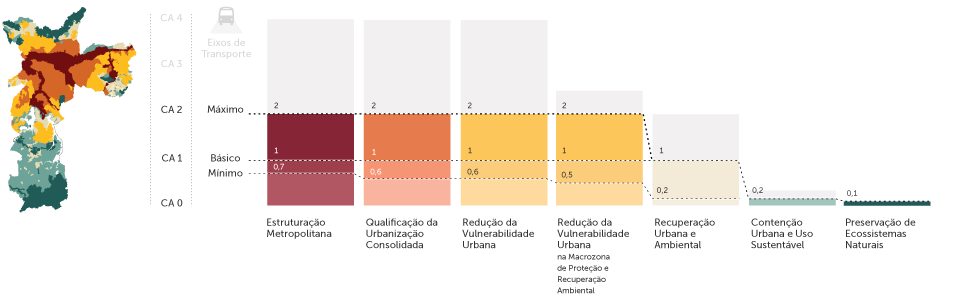
\includegraphics[width = \textwidth]{imagens/CA_macroareas.png}
    \end{subfigure}

    \caption*{\raggedright \textbf{Eixos de Estruturação da Transformação Urbana (EETU)}}
    \begin{subfigure}{.9\textwidth}
        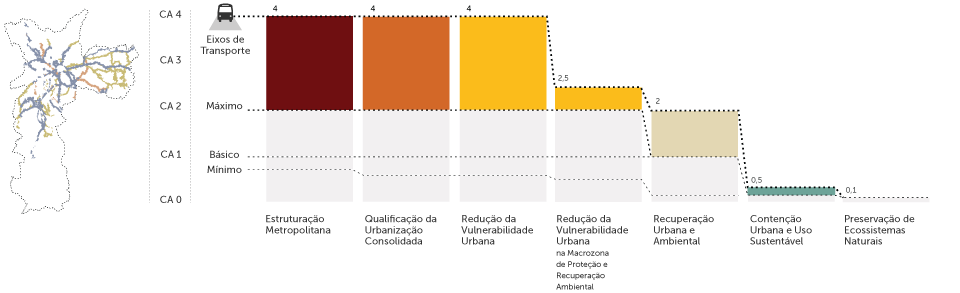
\includegraphics[width = \textwidth]{imagens/CA_eixos.png}
    \end{subfigure}
    \caption*{Fonte: \url{https://gestaourbana.prefeitura.sp.gov.br/marco-regulatorio/plano-diretor/entenda-o-projeto-de-lei-68813/}}
\end{figure}

Da mesma forma, existem parâmetros para a cota parte na cidade, a depender da localização. Nas Macrozonas de Estruturação e Qualificação Urbana, por exemplo, a cota parte apontada na Equação \ref{eq:cotaparte} como $Q$ equivale a 20. Em termos práticos, isso significa que um lote de 1.000m$^2$ hipotético deve apresentar no mínimo 50 unidades habitacionais. Este valor não é incrementado por um aumento do CA, mas pode decrescer se o CA escolhido pelo projeto seja menor do que o CA máximo da região.

Nesse sentido, não existe exatamente um dispositivo que determine a densidade populacional em si. Isso pode levar a um cenário em que o mercado está fracamente regulado, implicando que a densidade não está sendo efetivamente decidia pelo PDE. Apesar de haver um número mínimo de unidades habitacionais, estas não necessariamente se traduzem em população, dado que ao mesmo tempo que pode abrigar uma única pessoa, também pode abrigar uma família com diversos membros. Além disso, este valor mínimo não é afetado pela verticalização do imóvel, então imóveis com um CA maior não são obrigados a terem mais unidades habitacionais.

\subsection*{\textbf{O problema}}

Levando em consideração que um dos principais objetivos do PDE é estimular o adensamento de determinadas áreas, é importante avaliar se os instrumentos de regulação que estão disponíveis para alcançar este objetivo são eficientes. Em outras palavras, é crucial entender se os 3 components expostos (CA, cota parte e gabarito) são suficientes para determinar a densidade populacional que um novo empreendimento vai gerar. 

Caso estes instrumentos apontados não sejam eficientes em determinar a densidade, o nível de adensamento estaria sendo decidido pelo mercado. Entretanto, o que é importante notar é que o mercado sempre busca maximizar seus lucros, o que não necessariamente reflete em maior densidade populacional. Do ponto de vista teórico, é importante compreender quais elementos estão envolvidos nas escolhas das firmas na oferta de unidades de habitação, que será uma discussão da Seção \ref{sec:micro}.

Na Seção \ref{sec:emp}, será avaliado se estes instrumentos determinam a densidade demográfica. Para tanto, serão usados os dados do IPTU para calcular os indicadores utilizados na regulação e os dados do Censo de 2022, para identificar a densidade demográfica da região. Caso os indicadores sejam suficientes para explicar a densidade, significa que o PDE consegue definir a densidade usando os instrumentos previstos na lei. Caso contrário, a densidade populacional está sendo efetivamente decidida via mercado, não estando necessariamente alinhada com os objetivos do Plano para a cidade.

\chapter{Teórico}
\label{sec:micro}

Na literatura microeconômica há diversos modelos que tentam compreender as dinâmicas econômicas da cidade. Utilizando premissas formais e provas matemáticas, é possível resolver o modelo para algumas variáveis endógenas, como preço por metro quadrado na cidade, uso do solo, densidade populacional, entre outros \cite{papageorgiou2012essay, fujita1989urban}. A seguir será apresentado o modelo simplificado desenvolvido em \cite{brueckner2011lectures}, com o foco na variável densidade habitacional. O objetivo é compreender como o mercado se comportaria sem a intervenção da regulamentação e qual seria o seu impacto na variável resposta.

O modelo microeconômico começa com premissas simplificadoras fortes, mas que podem ser flexibilizadas na medida que algum componente merece ser discutido. Em sua primeira versão, a cidade é um círculo no qual todos os empregos se encontram no centro, as pessoas se deslocam uma distância ($x$) para trabalhar, o custo de transporte por distância é ($t$) e todos os moradores apresentam a mesma renda ($y$). A renda disponível é definida pela renda subtraída dos custos de transportes ($T=tx$). Por simplificação também, em cada unidade habitacional habita apenas uma pessoa. Nesse sentido, a densidade ($D$) é definida pelo número de unidades habitacionais por área.

Como o sistema está sempre em equilíbrio, todos os moradores apresentam a mesma utilidade em morar em cada ponto da cidade. Caso um lugar fosse melhor de morar, todos iriam querer se mudar para essa localização, aumentando seu preço ($p$). A função de utilidade dos cidadãos é composta por consumo de habitação ($q$) e outros bens, apelidados por pão, ($c$)\footnote{Por fins de simplificação, o preço do pão (outros bens) foi definido como unitário.}, de forma que toda sua renda disponível será gasta com estes bens, então $y-tx=c+pq$. Para o consumidor, sempre é melhor consumir unidades habitacionais maiores e mais pão, ou seja, quanto maior $p$ e $c$, maior sua utilidade. Dessa forma, quanto mais próximo do centro, e, portanto, um menor $x$, maior pode ser o gasto com $q$ e $c$.

Analogamente, os produtores também apresentam lucro igual para produção imobiliária em todos os pontos da cidade. Se algum lugar na cidade lucrasse mais do que outro, as firmas buscariam produzir lá e, portanto, seu preço reduziria com a expansão de oferta, equilibrando o sistema. Os produtores apresentam uma função de produção que depende do preço ($r$) da terra ($l$) e do custo ($i$) da verticalização ($N$). Se construir um novo andar em um terreno existente for mais barato que comprar um novo terreno, a incorporadora decidirá por verticalizar, mas a cada novo andar construído, o próximo apresentará um custo maior.

Com o modelo construído, agora é possível resolvê-lo de forma a descobrir o preço do metro quadrado na cidade. Na Figura \ref{fig:micro} é possível observar o que acontece com o preço por metro quadrado ($p$) na medida em que aumenta a distância ao centro ($x$). Como a renda é constante na cidade e os preços por metro quadrado são maiores no centro, os habitantes no centro conseguem comprar apartamentos menores. Dessa forma a densidade habitacional apresenta o mesmo comportamento do que o preço do metro quadrado: na medida em que aumenta $x$, $D$ reduz.

\begin{figure}[h]
    \centering
    \caption{Curva de preço por metro quadrado}
    \begin{subfigure}{.6\linewidth}
        \begin{tikzpicture}

    \begin{axis}[standard,
        xtick={0},
        ytick={0},
        xticklabels = {},
        yticklabels = {},
        samples=100,
        xlabel={Distância ao centro ($x$)},
        ylabel={\$},
        xmin=0,xmax=2,
        ymin=0,ymax=1,
        y label style={anchor=east},
        x label style={anchor=north},
    ]
    
\addplot[name path=F,domain={0:2}]{e^(-x)} node[pos=1] (point) {};
\node [right] at (point) {$p$};



    
\end{axis}
\end{tikzpicture}
    \end{subfigure}
    \label{fig:micro}
\end{figure}

Portanto, com essas premissas e resultados, não é necessária a intervenção do governo para regulamentar a densidade, visto que as próprias forças de mercado adensam as regiões centrais. Dessa forma, regulamentações podem mais gerar peso morto, ineficiência e burocracia. Entretanto, algumas das premissas do modelo são tão fortes, que o tornam descolado da realidade. Inclusive, o efeito da distância pode ser ambíguo na densidade a depender de algumas premissas. 
% Um exemplo disso é quando se incorpora no modelo níveis de renda diferentes.

Suponha uma cidade na qual os habitantes possuem mais de uma opção de meio de transporte. Os ricos, por exemplo, se deslocam de carro e os pobres, de ônibus. Como o carro apresenta um custo mais alto, esse grupo vai valorizar mais morar em regiões centrais, visto que o efeito da distância ($x$) em sua renda disponível é maior. Com este novo cenário, o quanto cada grupo está disposto a pagar pelo metro quadrado muda do cenário da Figura \ref{fig:micro} para a Figura \ref{fig:micro-2}, na qual se observa um padrão de segregação espacial dos dois grupos. Os ricos, que habitam o centro, possuem um maior poder aquisitivo, então vão consumir apartamentos maiores. Como consequência, têm-se que com essas novas premissas, a densidade habitacional no centro já não é mais tão grande.

\begin{figure}[h]
    \centering
    \caption{Curva de preço por metro quadrado com dois grupos}
    \begin{subfigure}{.6\linewidth}
        \begin{tikzpicture}

    \begin{axis}[standard,
        xtick={0},
        ytick={0},
        xticklabels = {},
        yticklabels = {},
        samples=100,
        xlabel={Distância ao centro ($x$)},
        ylabel={\$},
        xmin=0,xmax=2,
        ymin=0,ymax=1,
        y label style={anchor=east},
        x label style={anchor=north},
    ]
    
\addplot[name path=F,domain={0:2}]{e^(-x)} node[pos=1] (point1) {};
\node [right] at (point1) {$p_R$};

\addplot[name path=G,domain={0:2}]{0.5 * e^(-0.5*x) + .1} node[pos=1] (point2) {};
\node [right] at (point2) {$p_P$};

\path [name intersections={of=G and F, by = intersec}]; 
\draw[dashed] (intersec) -- (intersec|-{axis cs:0,0});

    
\end{axis}
\end{tikzpicture}
    \end{subfigure}
    \label{fig:micro-2}
\end{figure}


% Supondo agora uma cidade que possui dois grupos de renda, os ricos e os pobres. As outras premissas se mantém. Agora, se tanto os pobres quanto os ricos estiverem competindo pela mesma unidade habitacional, sempre vencerá quem consegue pagar o maior preço. Para determinar a localização que cada grupo se encontra na cidade, é importante comparar as curvas de preço, como da Figura \ref{fig:micro}, e analisar para cada parte da cidade, quem está disposto a pagar mais pela unidade habitacional.

% Várias hipóteses de como essas curvas se comportam podem surgir, a depender de como o componente renda é incorporado no modelo. Uma que é razoável para o Brasil

Com estas novas premissas, um tomador de decisão que tem como objetivo garantir maior densidade habitacional no centro deve intervir neste mercado, visto que a organização \textit{laisses-faire} leva a um equilíbrio menos denso do que o discutido no caso anterior. Nesse sentido, do ponto de vista microeconômico não é determinístico como o mercado se articula para definir a densidade habitacional.


\chapter{Dados}
\label{sec:emp}

\section*{Dados do Censo}

Para compreender o perfil geográfico da distribuição populacional de São Paulo foram utilizados os dados preliminares do Censo de 2022, feito pelo IBGE. Segundo o levantamento, a atual população do município de SP se encontra em 11.451.999 de habitantes, dividios em 4.996.529 de domicílios, dos quais apenas 4.316.336 estão ocupados. Na Figura \ref{fig:populacao} é possível observar quais são as áreas mais densas da cidade. A densidade foi calculada através da população no setor censitário dividida pela sua área. Os dados do censo foram utilizados em sua escala mais micro possível: nível setor censitário. 

\begin{figure}[!h]
    \centering
    \caption{Densidade populacional em São Paulo por setor censitário (Censo 2022)}
    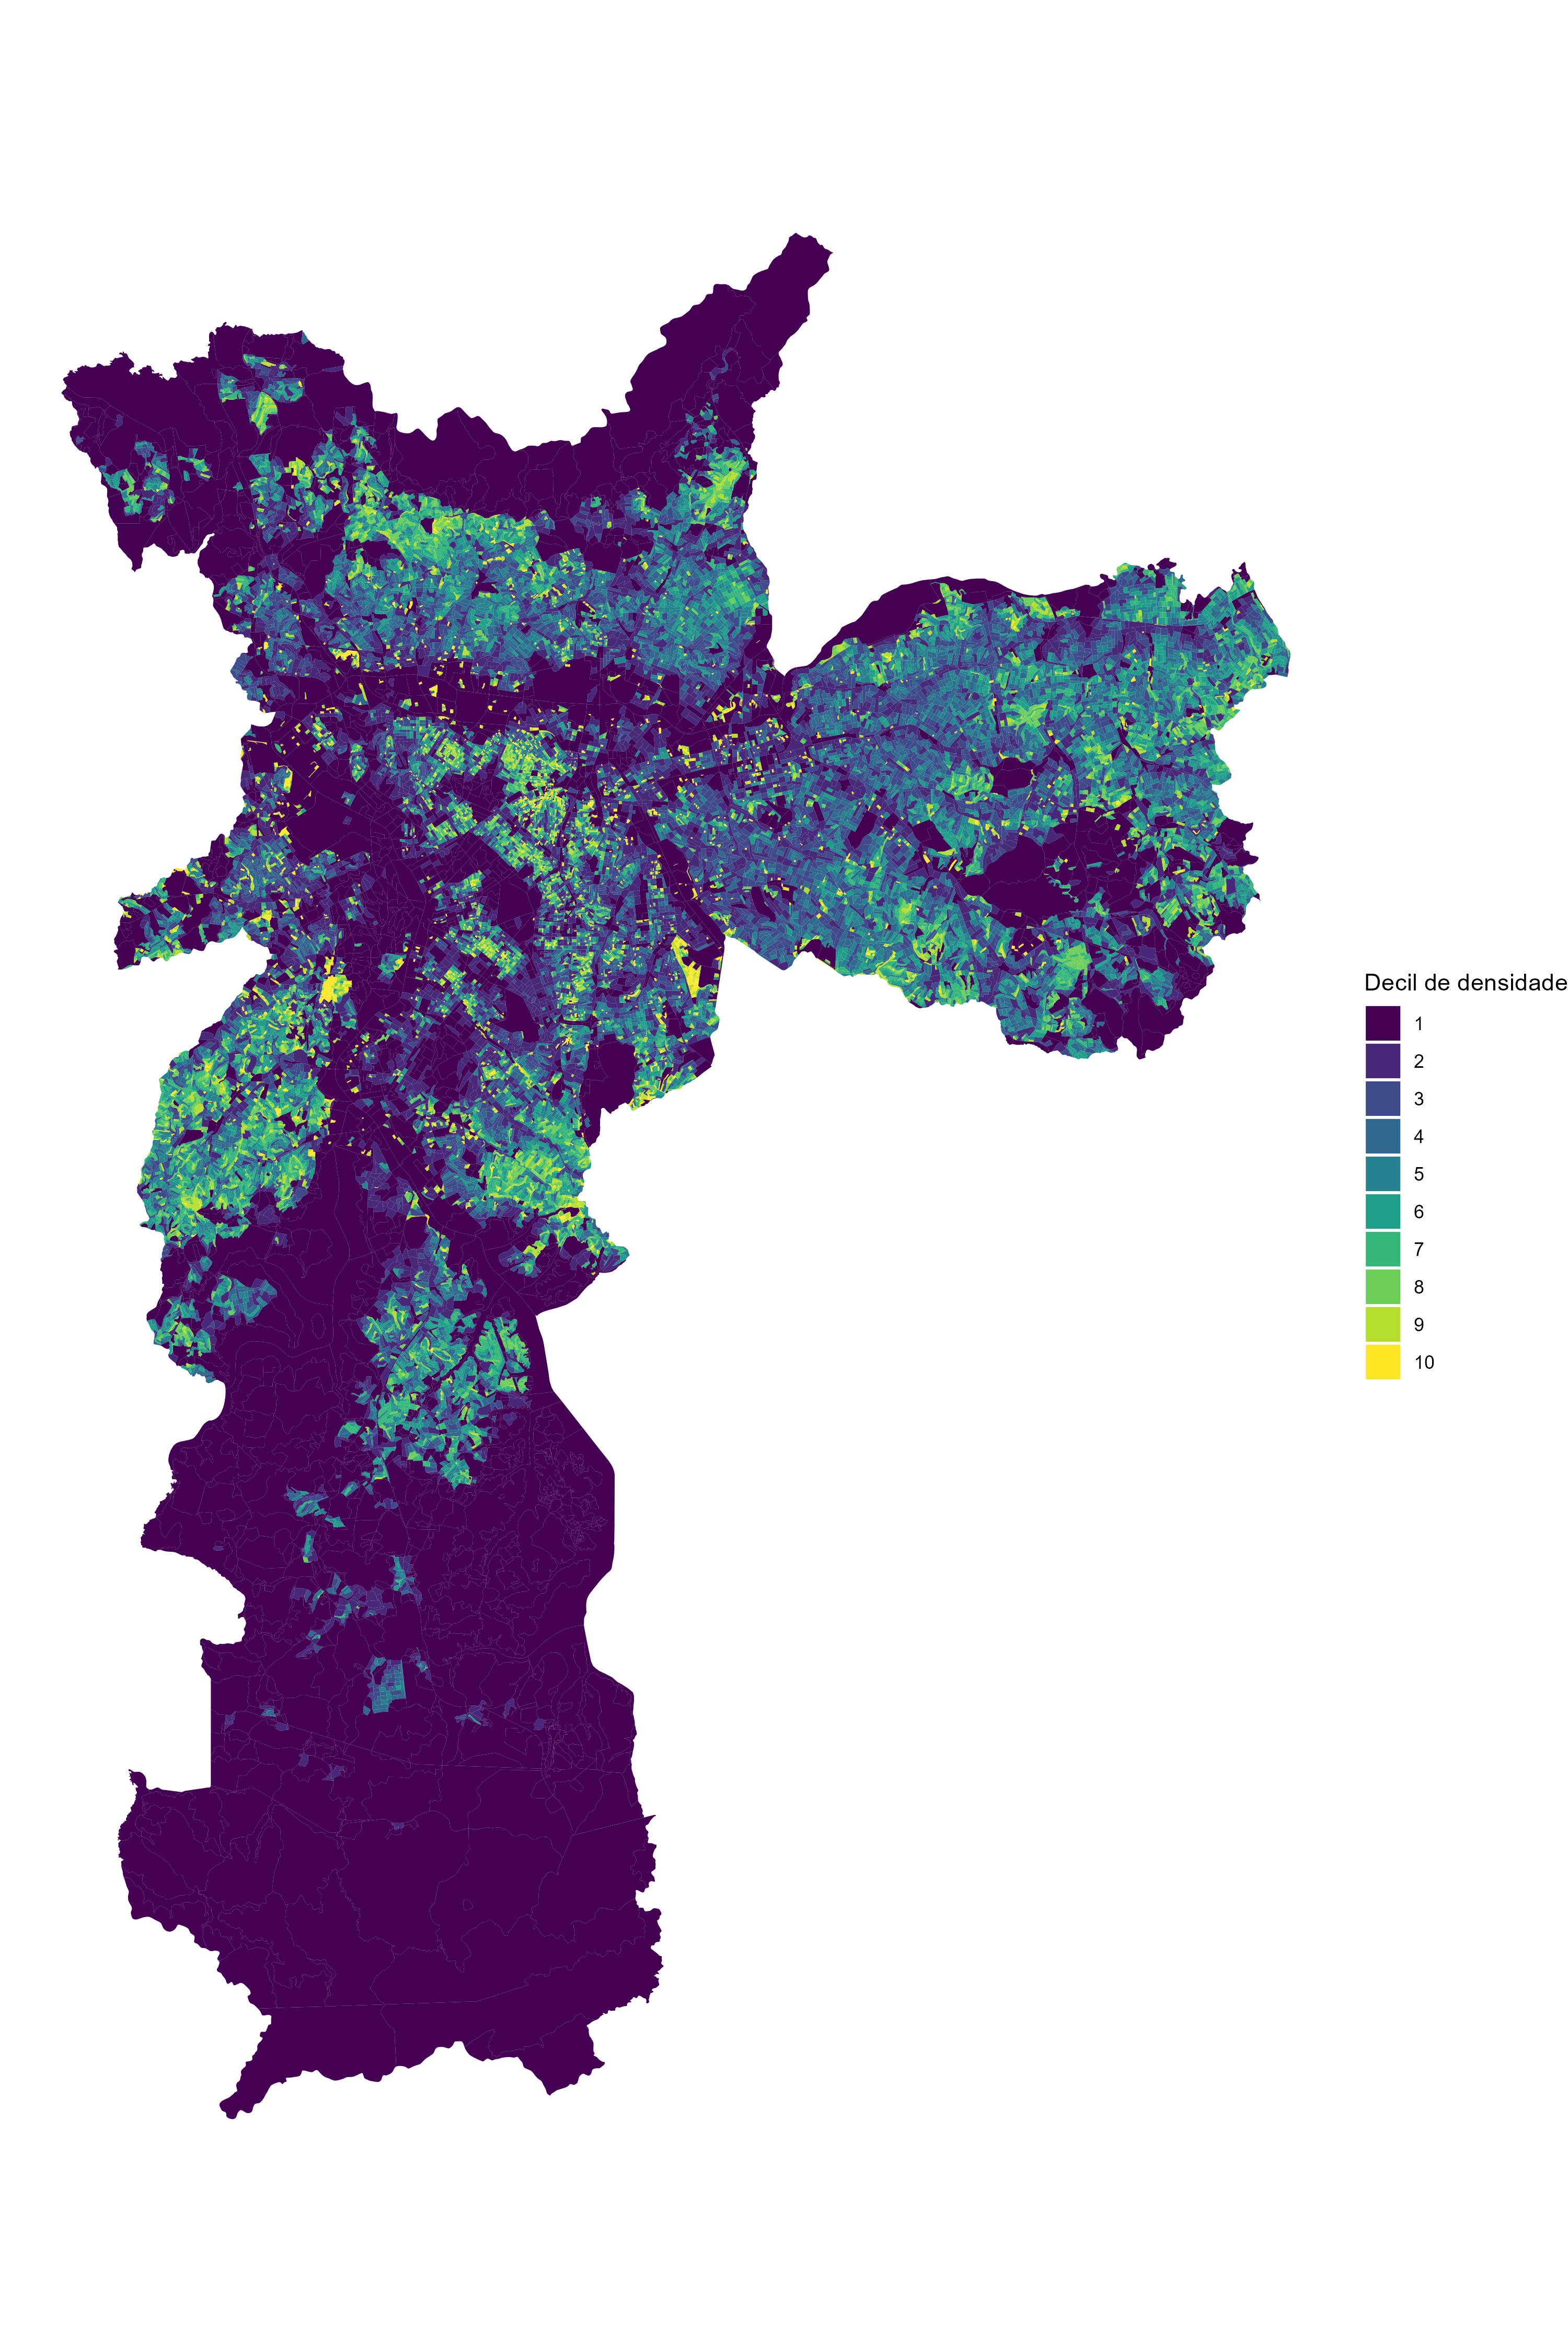
\includegraphics[width = .85\linewidth]{imagens/mapa.png}
    \label{fig:populacao}
\end{figure}

A metodologia para a delimitação dos setores censitários leva em consideração diversos fatores, como elementos na paisagem que se constituam em barreiras naturais ou artificiais e dificultam o trabalho do agente, pontos de referência estáveis e de fácil identificação no terreno, limites das estruturas territoriais, entre outros \cite{IBGE2024}. De maneira geral, estes limites são construídos de forma que o agente de coleta consiga cobrir o setor inteiro, minimizando os erros de medição. Estes setores censitários também são georreferenciados através da malha preliminar divulgada pelo IBGE e apresentam um número de identificação que pode ser decomposto segundo o exemplo apresentado a seguir.

\begin{equation*}
    \underbrace{21}_\text{UF} \underbrace{00873}_\text{Município} \underbrace{05}_\text{Distrito} \underbrace{00}_\text{Subdistrito} \underbrace{0026}_\text{Setor} \underbrace{P}_\text{Preliminar}
    \label{eq:setor}
\end{equation*}

É interessante notar na Figura \ref{fig:populacao}, que o clássico modelo, no qual população se concentra principalmente no centro apresenta mérito, dado que perto da região da Sé, centro histórico de São Paulo, há uma enorme concentração habitacional. Entretanto, é surpreendente a densidade habitacional nas favelas de Paraisópolis e Heliópolis, que acabam por ser as áreas mais densas da cidade. Na Figura \ref{fig:dens-distcentro} é possível ver como ainda que haja uma relação entre a densidade habitacional e a distância, ela não é tão perfeita quanto no modelo microeconômico. Paraisópolis, por exemplo, está a 15km do centro e ainda é a região mais densa de São Paulo -- mais detalhes serão discutidos adiante.

\begin{figure}[h]
    \centering
    \caption{Densidade habitacional na medida em que se distancia da Sé}
    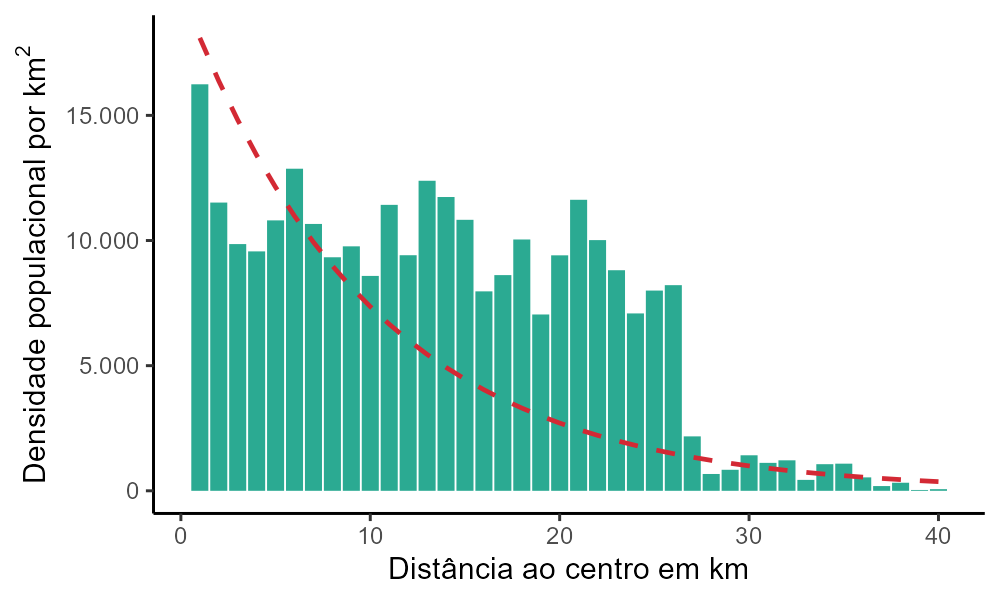
\includegraphics[width = .75\linewidth]{imagens/densidade_distcentro.png}
    \label{fig:dens-distcentro}
\end{figure}

\section*{Dados do IPTU}

Em relação aos dados sobre os empreendimentos imobiliários, a base de dados escolhida foi do IPTU. Para os fins deste artigo, ela é a mais completa, visto que não representa um fluxo de novos imóveis construídos todos os anos como a base da Embraesp, mas apresenta um estoque imobiliário de tudo que já foi construído legalmente na cidade. Dito isso, estão cadastrados os 3.096.719 números únicos de contribuintes, que, segundo a definição da documentação dos dados no GeoSampa, ``A cada imóvel urbano corresponderá um número de inscrição no Cadastro Imobiliário Fiscal, entendendo-se como imóvel: I - a área de terreno, construído ou não, definida em matrícula do competente Serviço de Registro de Imóveis ou em transcrições ainda vigente''. Os únicos dados que não constam nessa base são relativos a lotes irregulares ou não registrados, como em áreas de favelas. Estes casos podem ser visualizados na Figura \ref{fig:erros-join}, mas serão discutidos a seguir. Isso não é uma limitação, visto que os intrumentos de regulação urbana não se aplicam as estas áreas de qualquer forma.

Entre os dados disponíveis do IPTU, se destacam a área do terreno, a área construída, a área ocupada e o número de pavimentos do empreendimento. O tipo de uso do imóvel também está disponível, mas como esta pesquisa foca em densidade habitacional, foram descartados os usos não residenciais. Na figura \ref{fig:area_construida}, é possível observar a área construída por tipo e padrão de uso em São Paulo. Logo, com estes dados é possível calcular os indicadores utilizados pela regulamentação do coeficiente de aproveitamento (CA), gabarito e cota parte. A distribuição destes indicadores pode ser vista na Figura \ref{fig:histogramas}.

\begin{figure}[h]
    \centering
    \caption{Área construída em São Paulo por tipo e padrão de uso}
    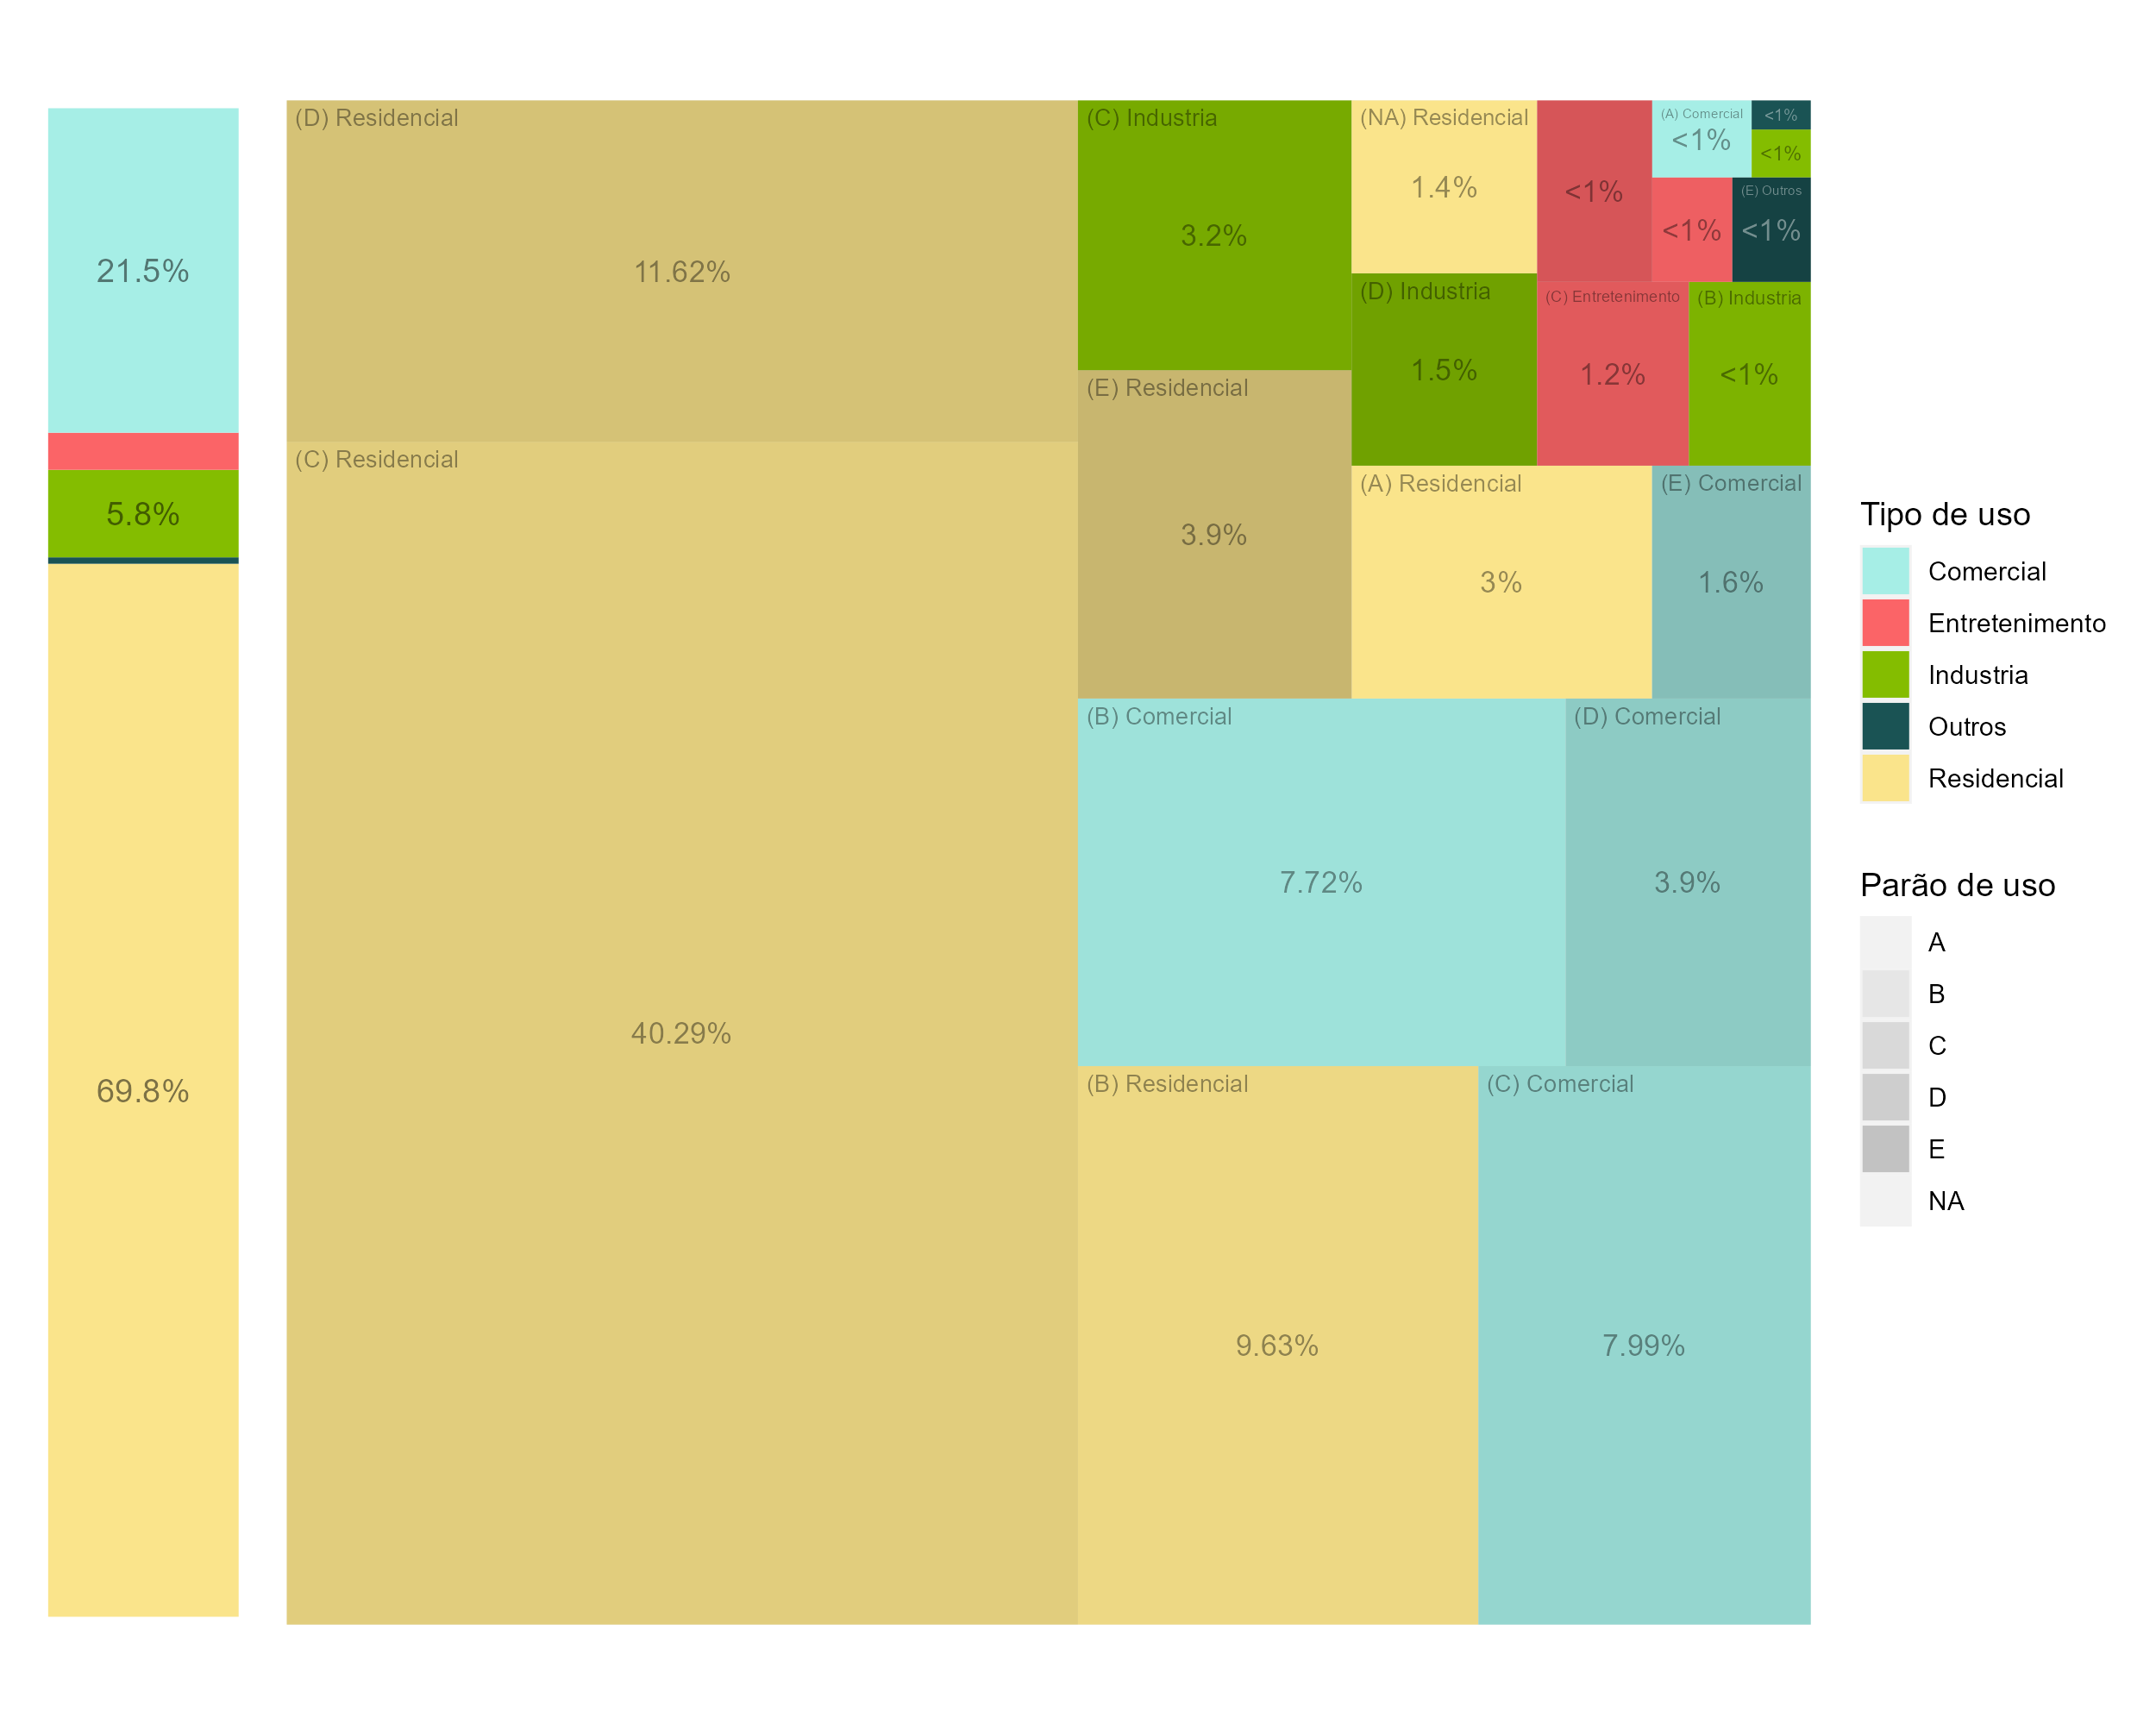
\includegraphics[width = .8\linewidth]{imagens/tree_area_construida.png}
    \label{fig:area_construida}
\end{figure}

Em São Paulo, 70\% da área construída é residencial, sendo que o padrão residencial mais comum é o "C". O padrão é uma divisão feita no cálculo do IPTU \cite{lei10235_1986}, para criar descontos do imposto para imóveis com características desejáveis do ponto de vista do planejamento urbano, como maior adensamento. Medidas como metragem, pé direito, vaga de garagem, número de pavimentos, elementos arquitetônicos, materiais de construção, etc., são fatores levados em consideração para determinar o padrão. No caso do "C", ele está no meio da escala de densidade, sendo "A" o mais denso, e "E" o menos. O segundo uso mais comum é o comercial, seguido do industrial e entretenimento. Na categoria de entretenimento encontram templos religiosos, clubes, estádios esportivos, cinemas, aeroporto, museu, zoológico, entre outros.

\begin{figure}[h]
    \centering
    \caption{Distribuição dos indicares em cada lote de São Paulo}
    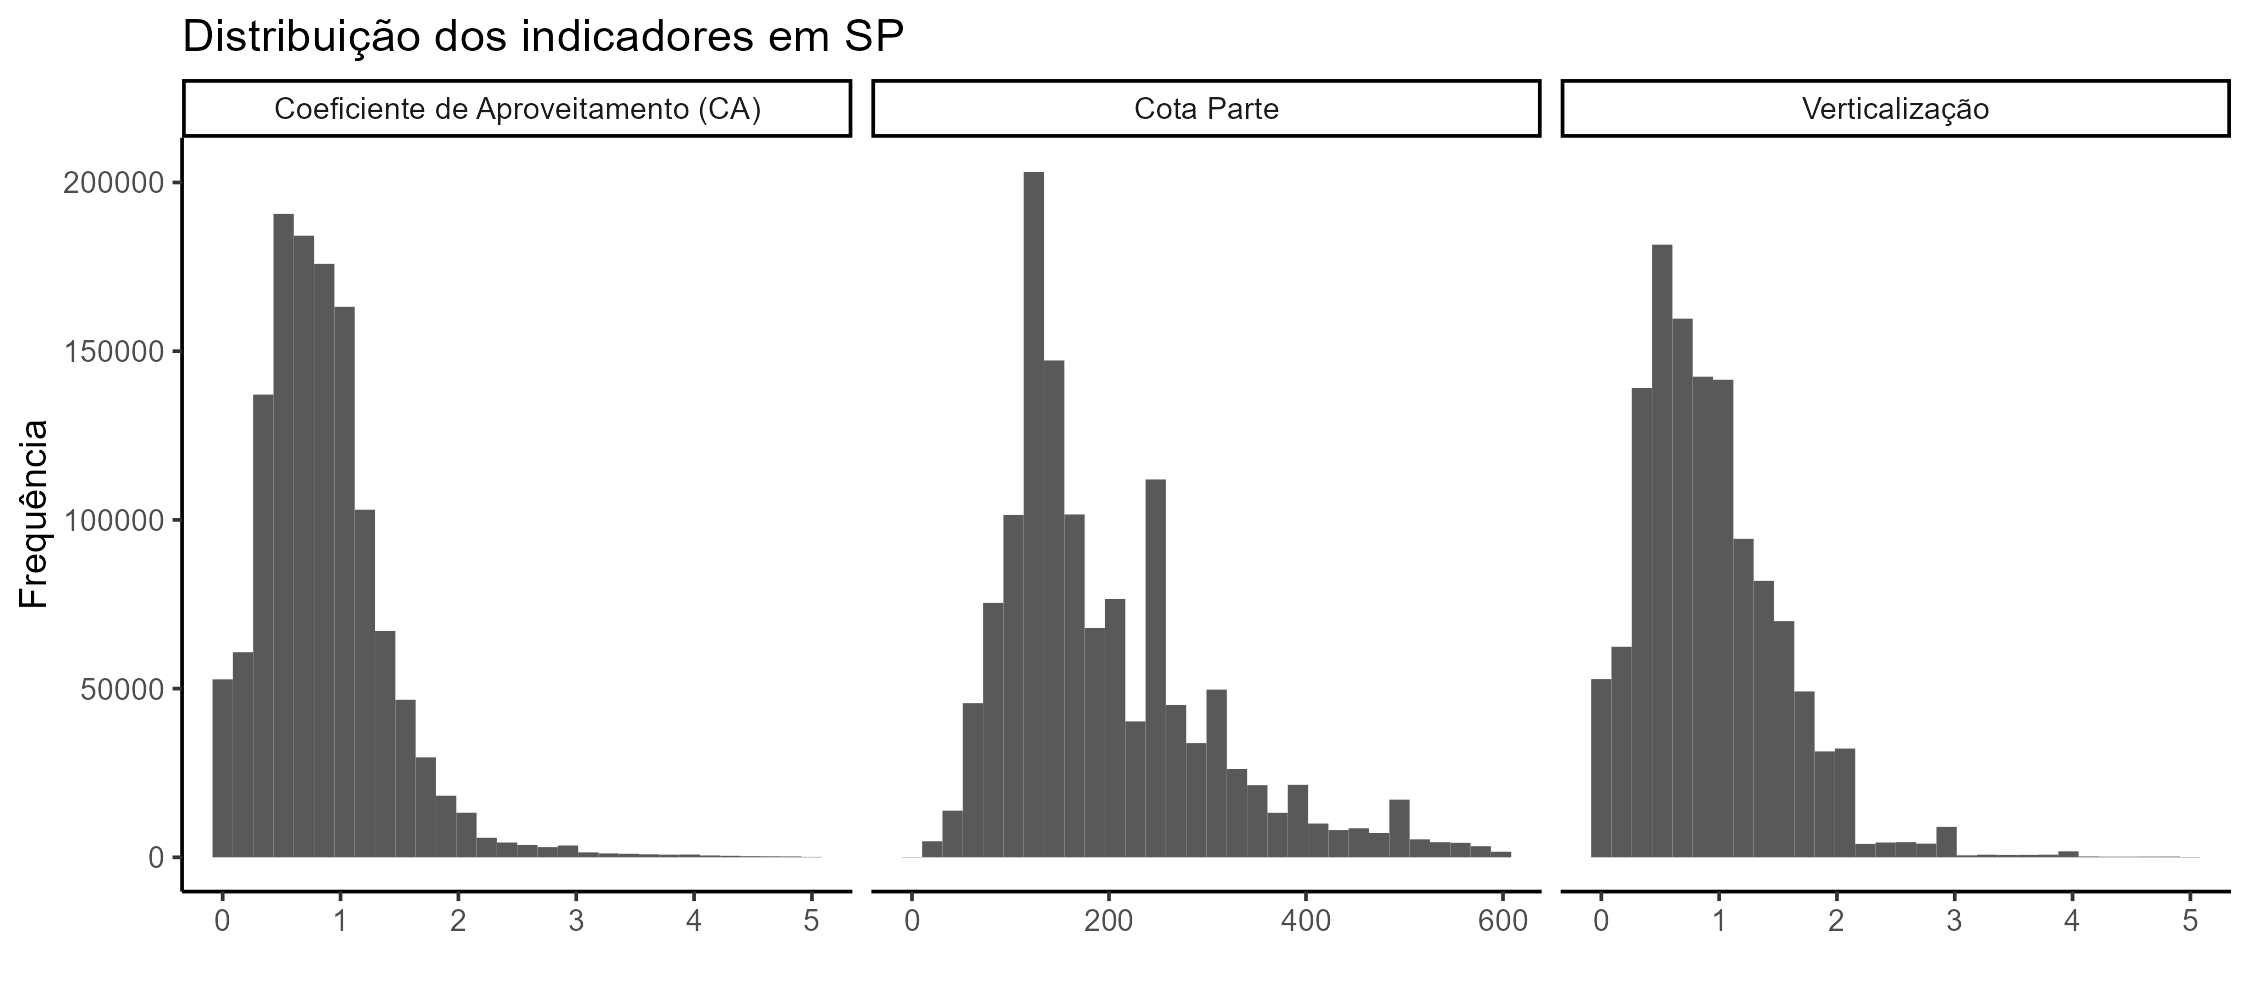
\includegraphics[width = \linewidth]{imagens/indicadores.png}
    \label{fig:histogramas}
\end{figure}

De fato, ao observar os indicadores na Figura \ref{fig:histogramas}, é possível notar que o perfil habitacional de São Paulo é bastante horizontal. É surpreendente que 95\% dos lotes residenciais em São Paulo apresentam 2 ou menos pavimentos. Ainda, a mediana do CA é 0,8, o que indica que em mais da metade dos lotes da cidade foi construído menos do que a área do terreno. Ainda, a cota parte mediana dos lotes da cidade é de 155$m^2$, o que representa um uso do terreno para poucas unidades habitacionais em média. 

\begin{figure}[h]
    \centering
    \caption{Variação no tempo dos indicadores residenciais em São Paulo}
    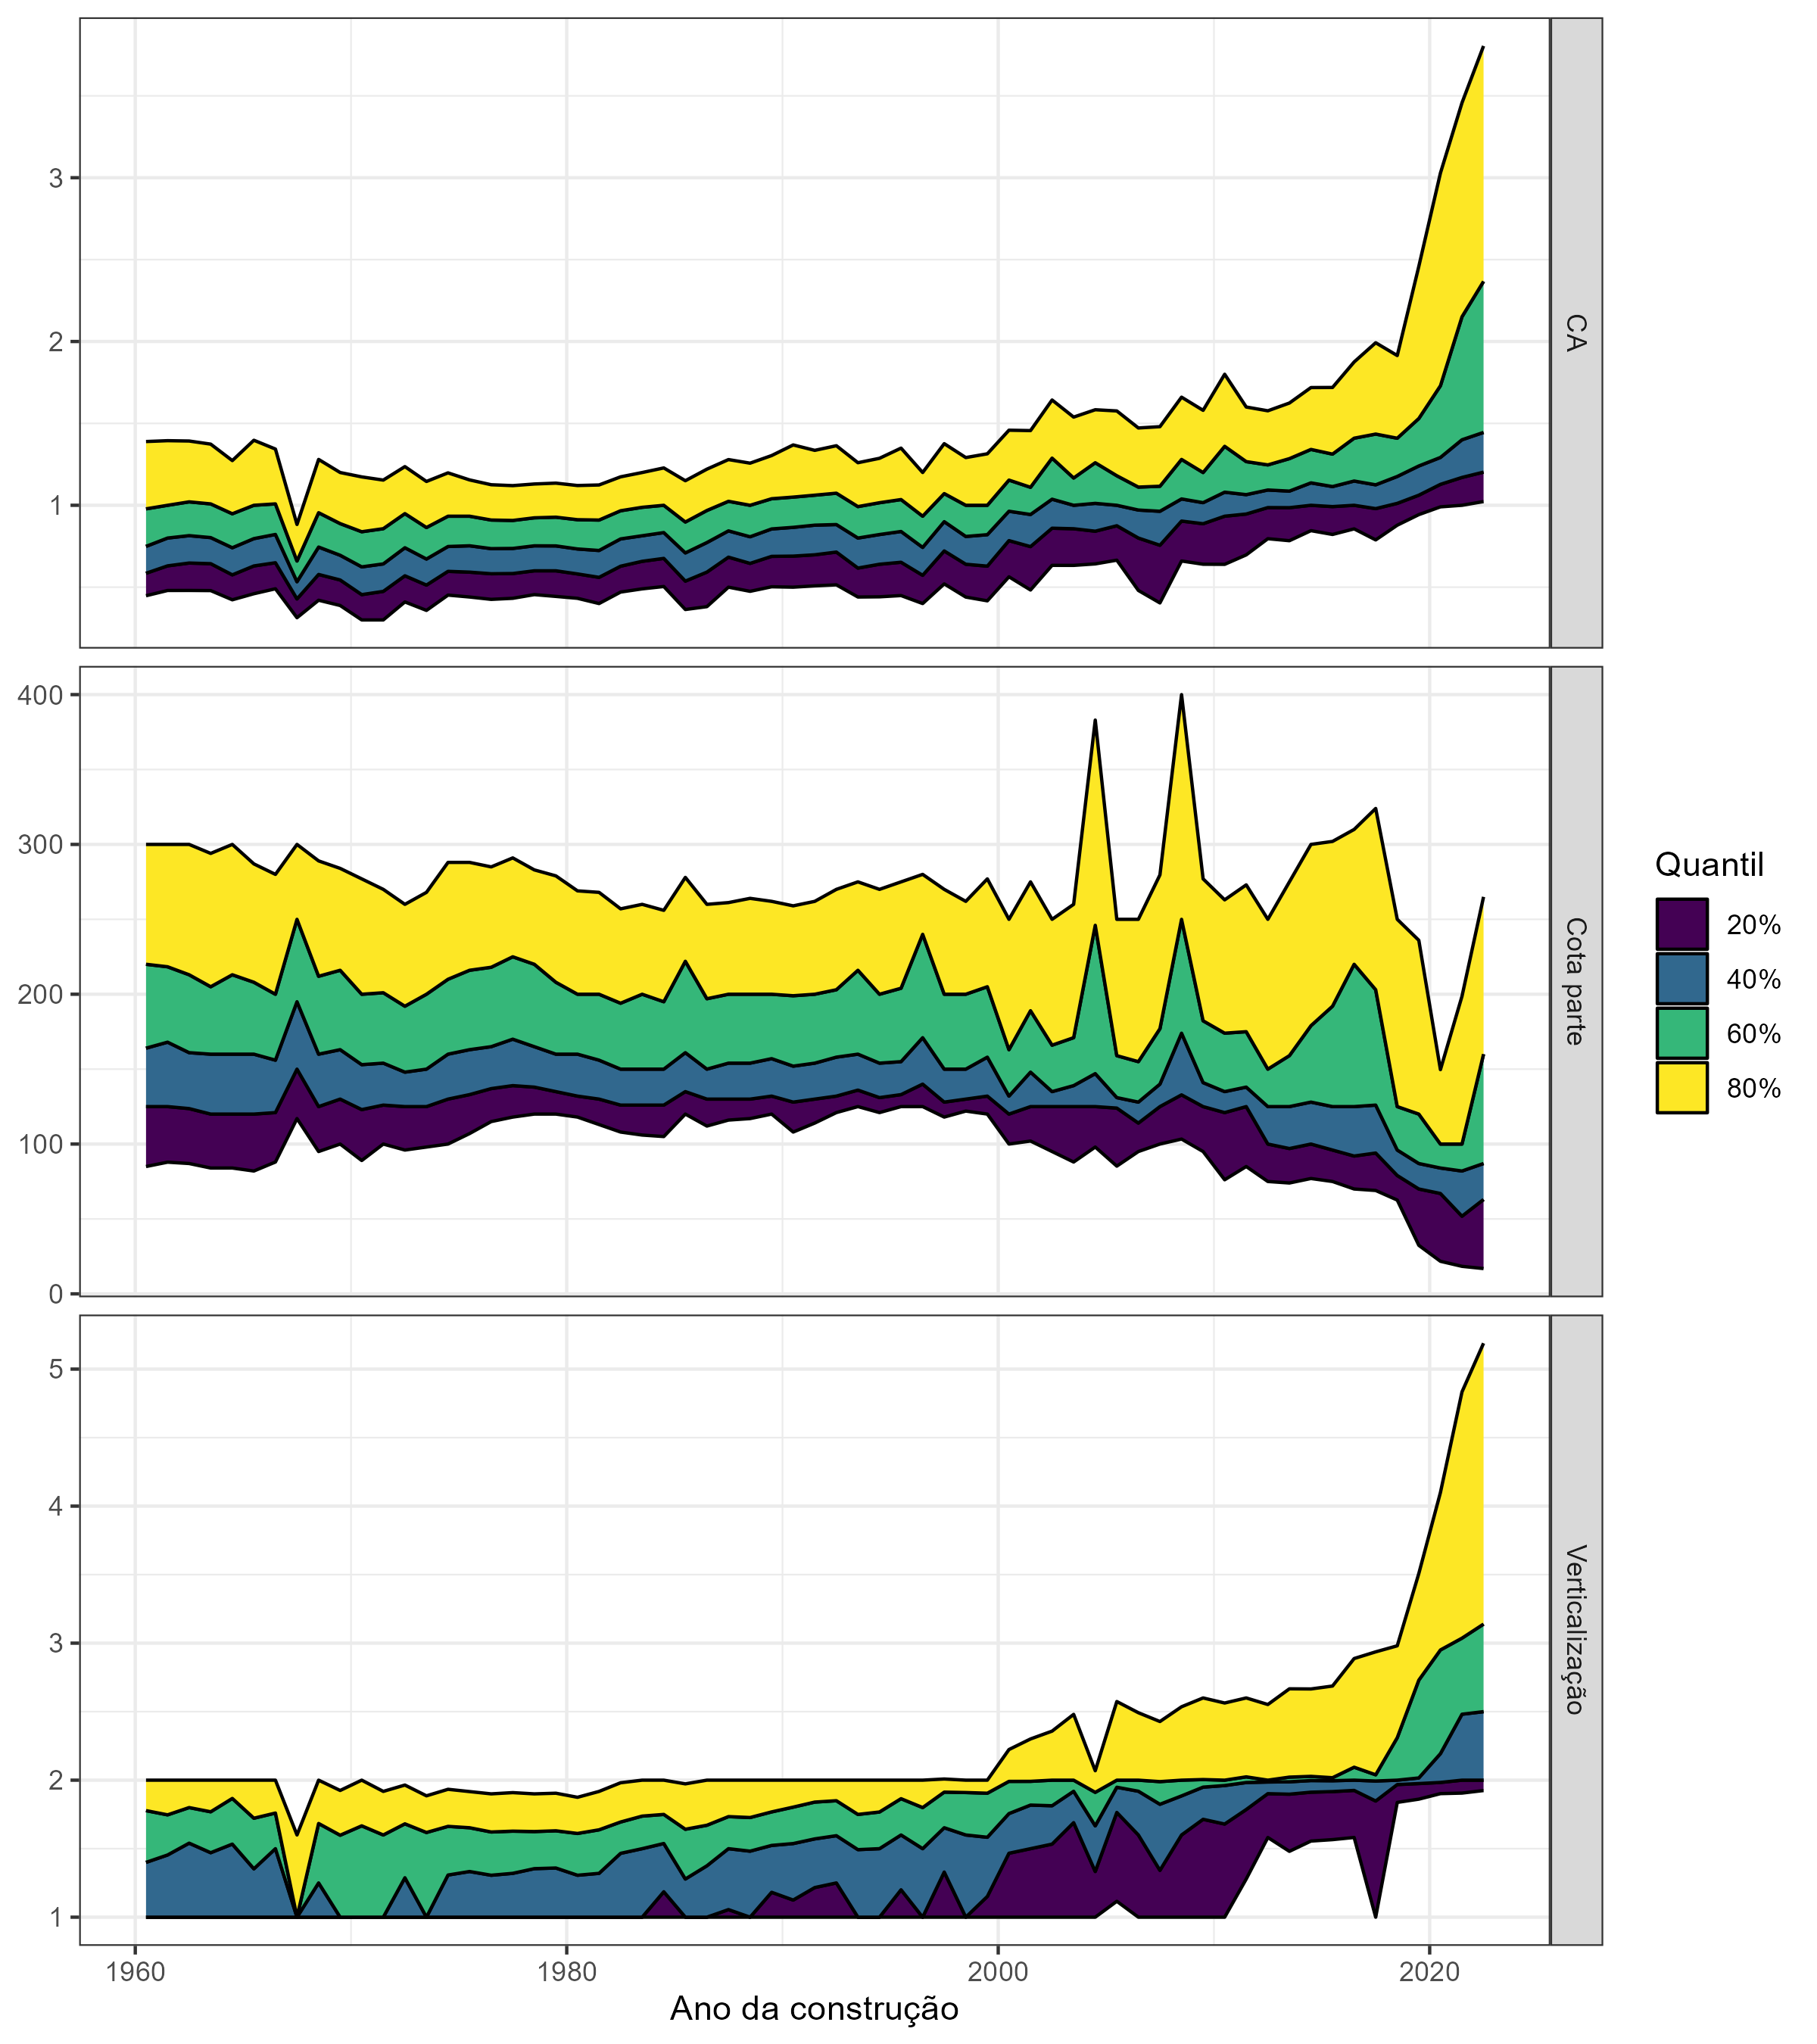
\includegraphics[width = \linewidth]{imagens/indicadores_tempo.png}
    \label{fig:indicadores-tempo}
\end{figure}

Todavia, ao analisar estes indicadores ao longo do tempo na Figura \ref{fig:indicadores-tempo}, fica evidente a trajetória de adensamento. Na figura, cada linha representa um quantil dos lotes do IPTU. Ao ordenar as construções no ano 2020 de maneira crescente de CA, observa-se que o empreendimento na posição 80\% dessa fila apresenta um CA de 3,8. Este mesmo procedimento nos anos 2000 retornaria um empreendimento com CA igual a 1,46. Analogamente, a cota parte que em 2020 apresenta o quantil 20\% de meros 21,7 metros quadrados, em 2000 apresentaria 100 metros quadrados. Isso evidencia que nos últimos anos São Paulo passou por um forte processo de adensamento.

\section*{Cruzamento dos dados}

Todavia, os dados do IPTU não são georreferenciados, então desacompanhados de outros dados não é possível cruzá-los com os do censo. O que possibilita fazer essa junção é que o número único de contribuinte, também é o código do Setor, Quadra e Lote (SQL) que o empreendimento se encontra. Nesse sentido, é possível decompor o SQL e cruzar com as bases de lotes, quadras e setores do GeoSampa, que contêm a geometria de cada  um dos 1.677.980 lotes, 45.987 quadras e 309 setores da cidade. O que explica a diferença entre o número de lotes e número de números dos contribuintes são os lotes que contém um condomínio, que pode haver diversos números únicos de contribuintes em apenas um lote. Nos dados de IPTU, há 1.314.353 contribuintes em lotes com apenas uma unidade habitacional e 33.129 condomínios, que contêm 1.782.366 unidades. Ao cruzar o SQL do IPTU com a base de lotes, 44.319 contribuintes não encontram um par na outra base, o que representa uma perda de 1,67\% das unidades. Caso o join seja feito com a base de quadras, a perda passa a ser de 820 contribuintes, um erro de 0,03\%. Já quando são cruzados com base no setor, o erro chega a 0.

Agora, com os dados do censo georreferenciados e os dados do IPTU também georreferenciados, é necessário juntar estas bases. Entretanto, como o recorte dos setores censitários não respeita os recortes dos lotes, algum tipo de critério deve ser adotado para conectar essas geometrias. Duas abordagens foram feitas, a primeira com um join geográfico e a segunda, a partir da rasterização de ambos os dados. Na primeira, para cada um dos 27.592 setores censitários foram identificados todos os lotes que se interseccionam com os setores. A partir disso, foram cortados os lotes que não estão contidos apenas em um setor, de forma a atribuir seus dados a todos os setores que pertence, ponderado pelo percentual de sua área que intersecciona com cada setor. A segunda abordagem envolve dividir a cidade em um quadriculado (\textit{raster}) e converter tanto os dados do IPTU quanto do censo para esta escala. A metodologia é parecida, visto que formado o quadriculado, os lotes são dividos entre cada quadrado, ponderando-se pelo percentual de sua área que intersecciona com cada um.

Dessa forma, para cada setor censitário ou para cada célula do raster, há varios lotes, que devem ser agregados segundo algum critério. Para a área construída, área ocupada, área do terreno e unidades, os valores de cada lotes podem ser simplesmente somados. Entretanto, no caso da verticalização fica mais complicado. A primeira possibilidade, de fazer uma média dos pavimentos, é bastante problemática, visto que se um lote fosse cortado no meio, tornando-se dois lotes e mantiver a construção com o mesmo número de pavimentos, a medida de verticalização vai se alterar, o que é um problema. A mediana também não funciona bem, visto que um local, por exemplo, com três lotes com diferentes pavimentos: 1, 3 e 10; e outro com 1, 3 e 30, vão apresentar a mesma verticalização. Caso a medida de verticalização seja uma média ponderada pela área ocupada, é possível que ao construir novos pavimentos em um terreno antes desocupado, haja uma redução na verticalização, caso esse número de pavimentos seja menor do que a média ponderada antes deste choque. 

O critério adotado nessa pesquisa foi de multiplicar o número de pavimentos pela taxa de ocupação do terreno (área ocupada / área do terreno) somado a (1 - taxa de ocupação) por zero pavimentos, Equação \ref{eq:verticaliz}. Depois, basta fazer uma média ponderada pelo tamanho do terreno desse índice de verticalização. Com este indicador, sempre que for construído algum pavimento, a verticalização vai aumentar e se um lote for cortado no meio, o índice não vai mudar. O único problema desse método é que o resultado acaba sendo muito parecido com o CA, visto que a área ocupada vezes o número de pavimentos é bastante parecida com a área construída, que ao ser dividida pela área do terreno é igual ao CA. Entretanto essa relação não é perfeita e a correlação entre o CA e a verticalização seguindo este método é de 83\% no caso da metodologia de join e 92\% na metodologia de \textit{raster}. A partir deste critério, CA e verticalização são variáveis um pouco redundantes, mas outras formas de calcular essa verticalização se mostraram mais problemáticas.

\begin{equation}
    \text{Verticalização} = \text{Pavimentos} * \frac{\text{Área Ocupada}}{\text{Área do Terreno}} + 0 * \frac{\text{Área não Ocupada}}{\text{Área do Terreno}}
    \label{eq:verticaliz}
\end{equation}


\begin{figure}
    \caption{Inconsistências entre dados do IPTU e do censo}
    \begin{subfigure}[t]{0.45\linewidth}
        \centering
        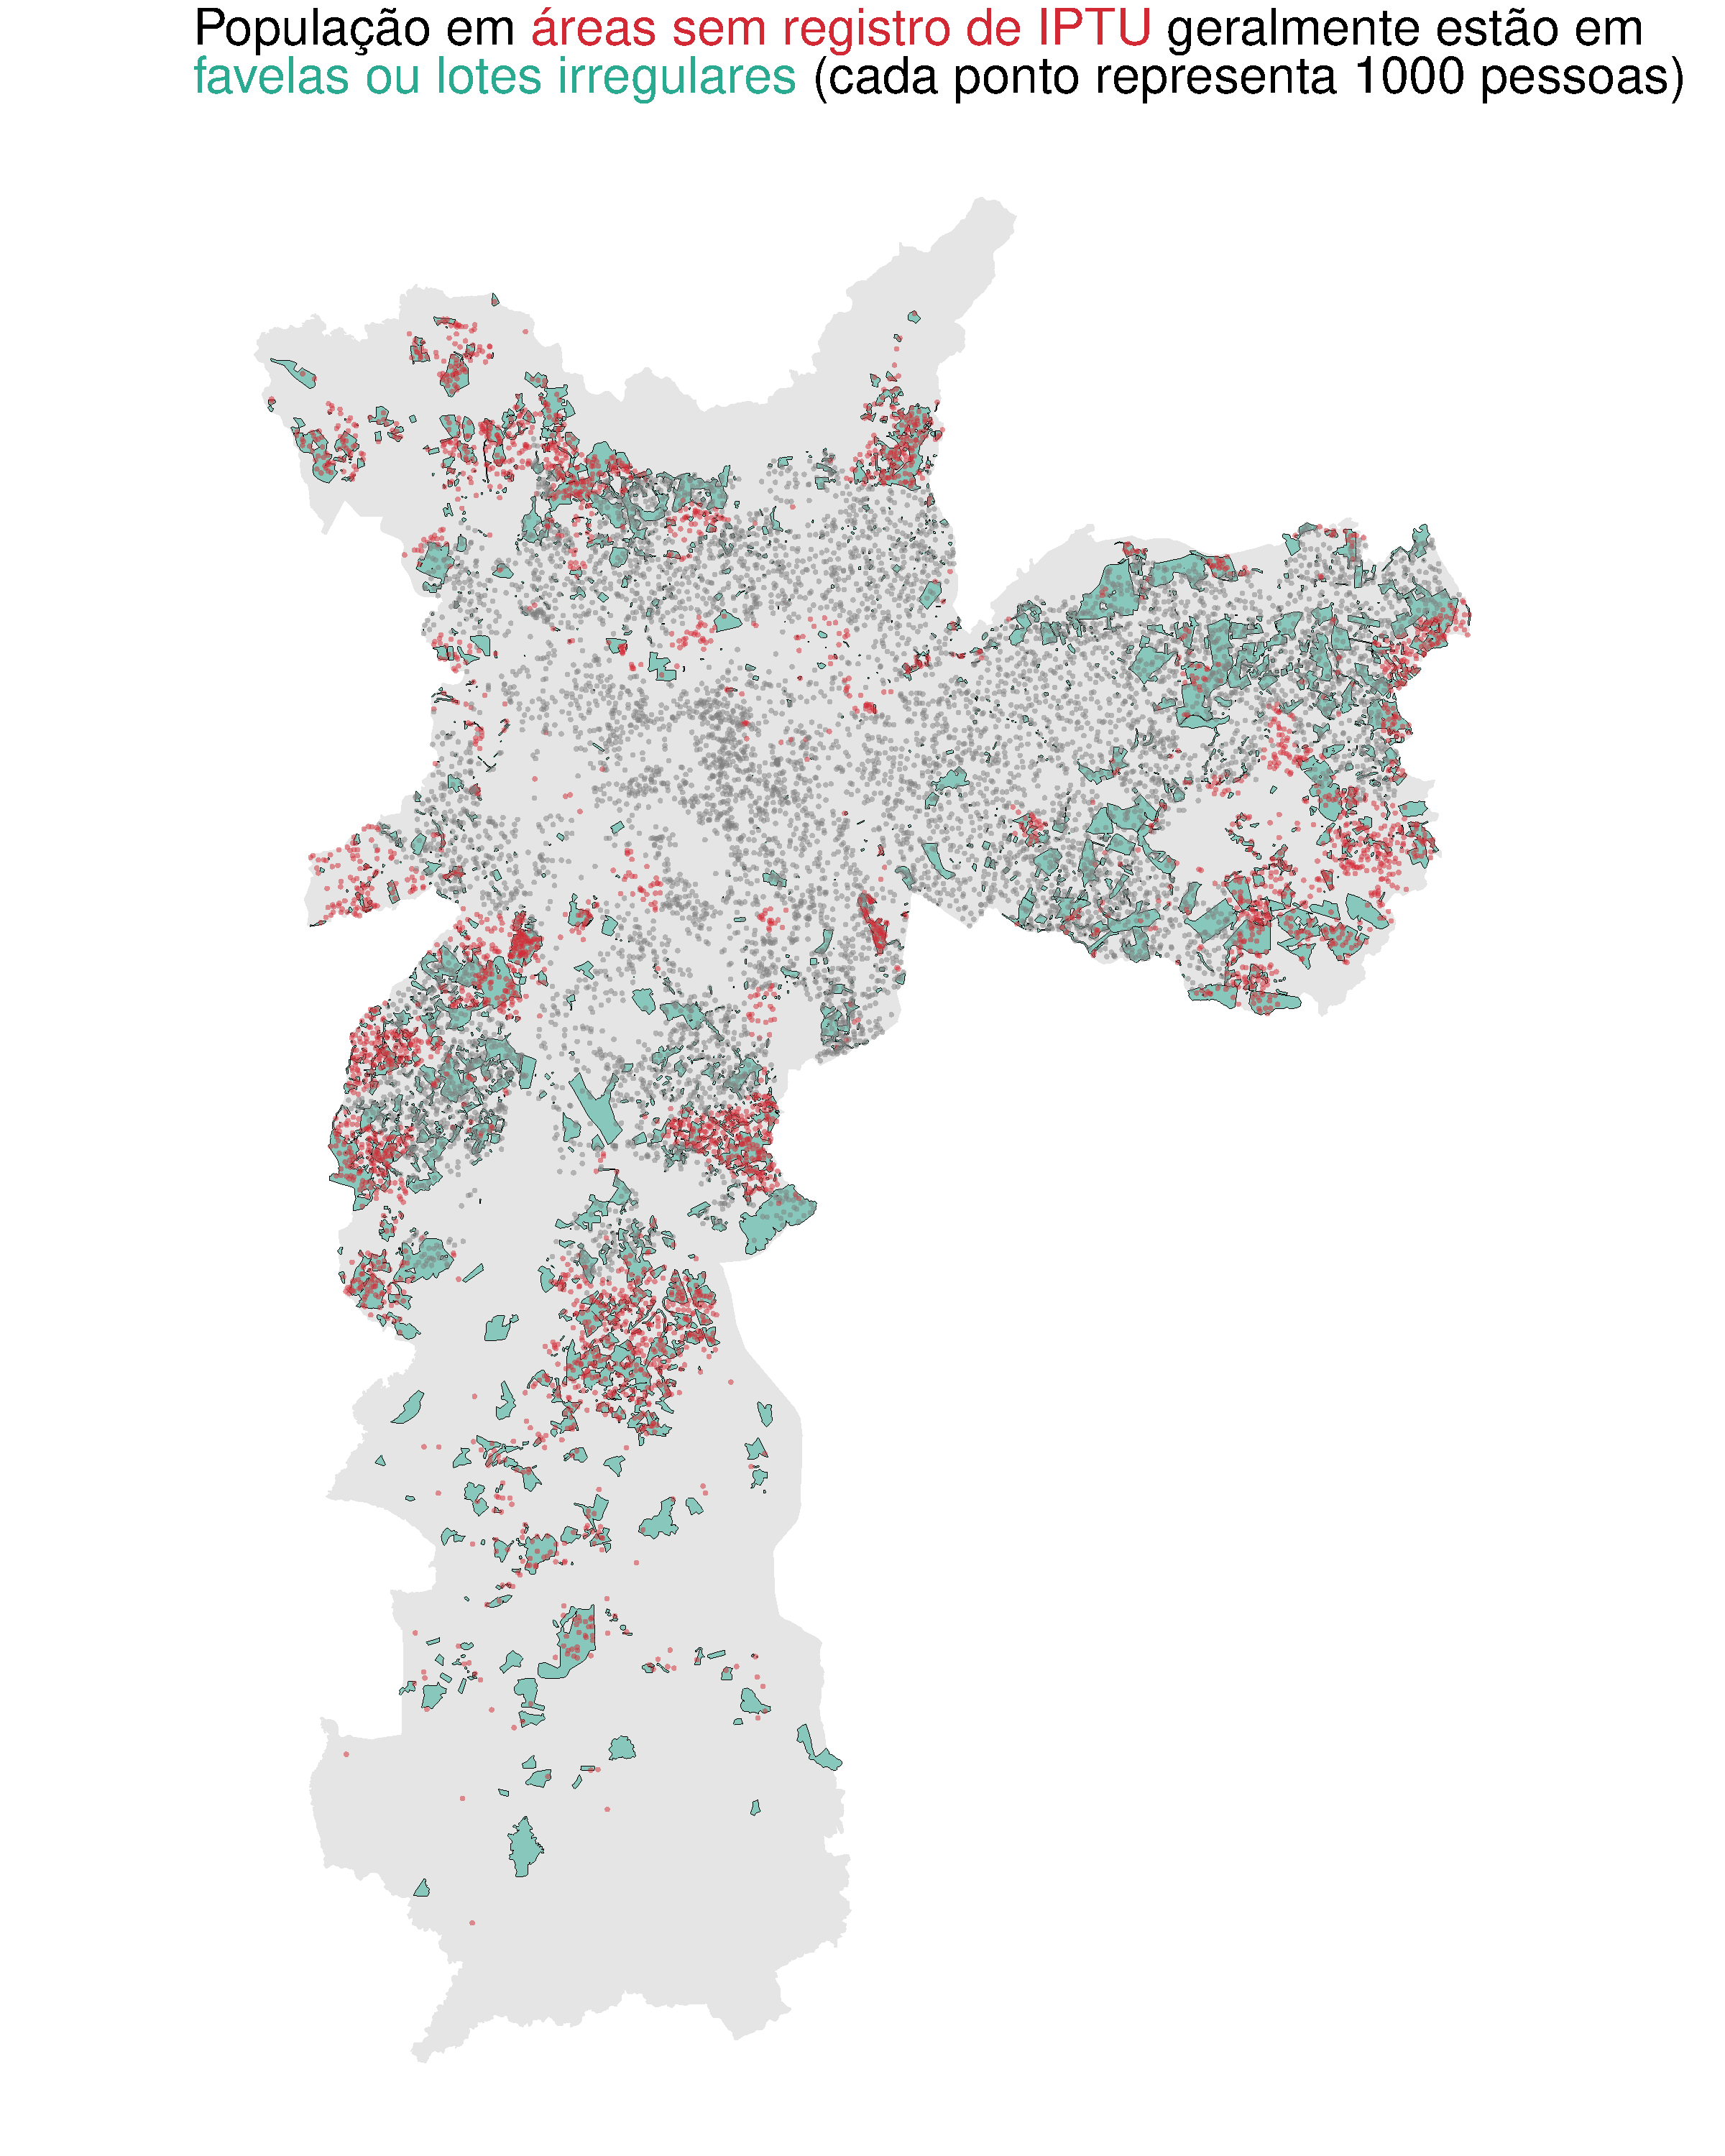
\includegraphics[width = \linewidth]{imagens/mapa_pontos.png}
        \caption{Abordagem join}
        \label{fig:pontos_erro}
    \end{subfigure}
    \hfill
    \begin{subfigure}[t]{0.45\linewidth}
        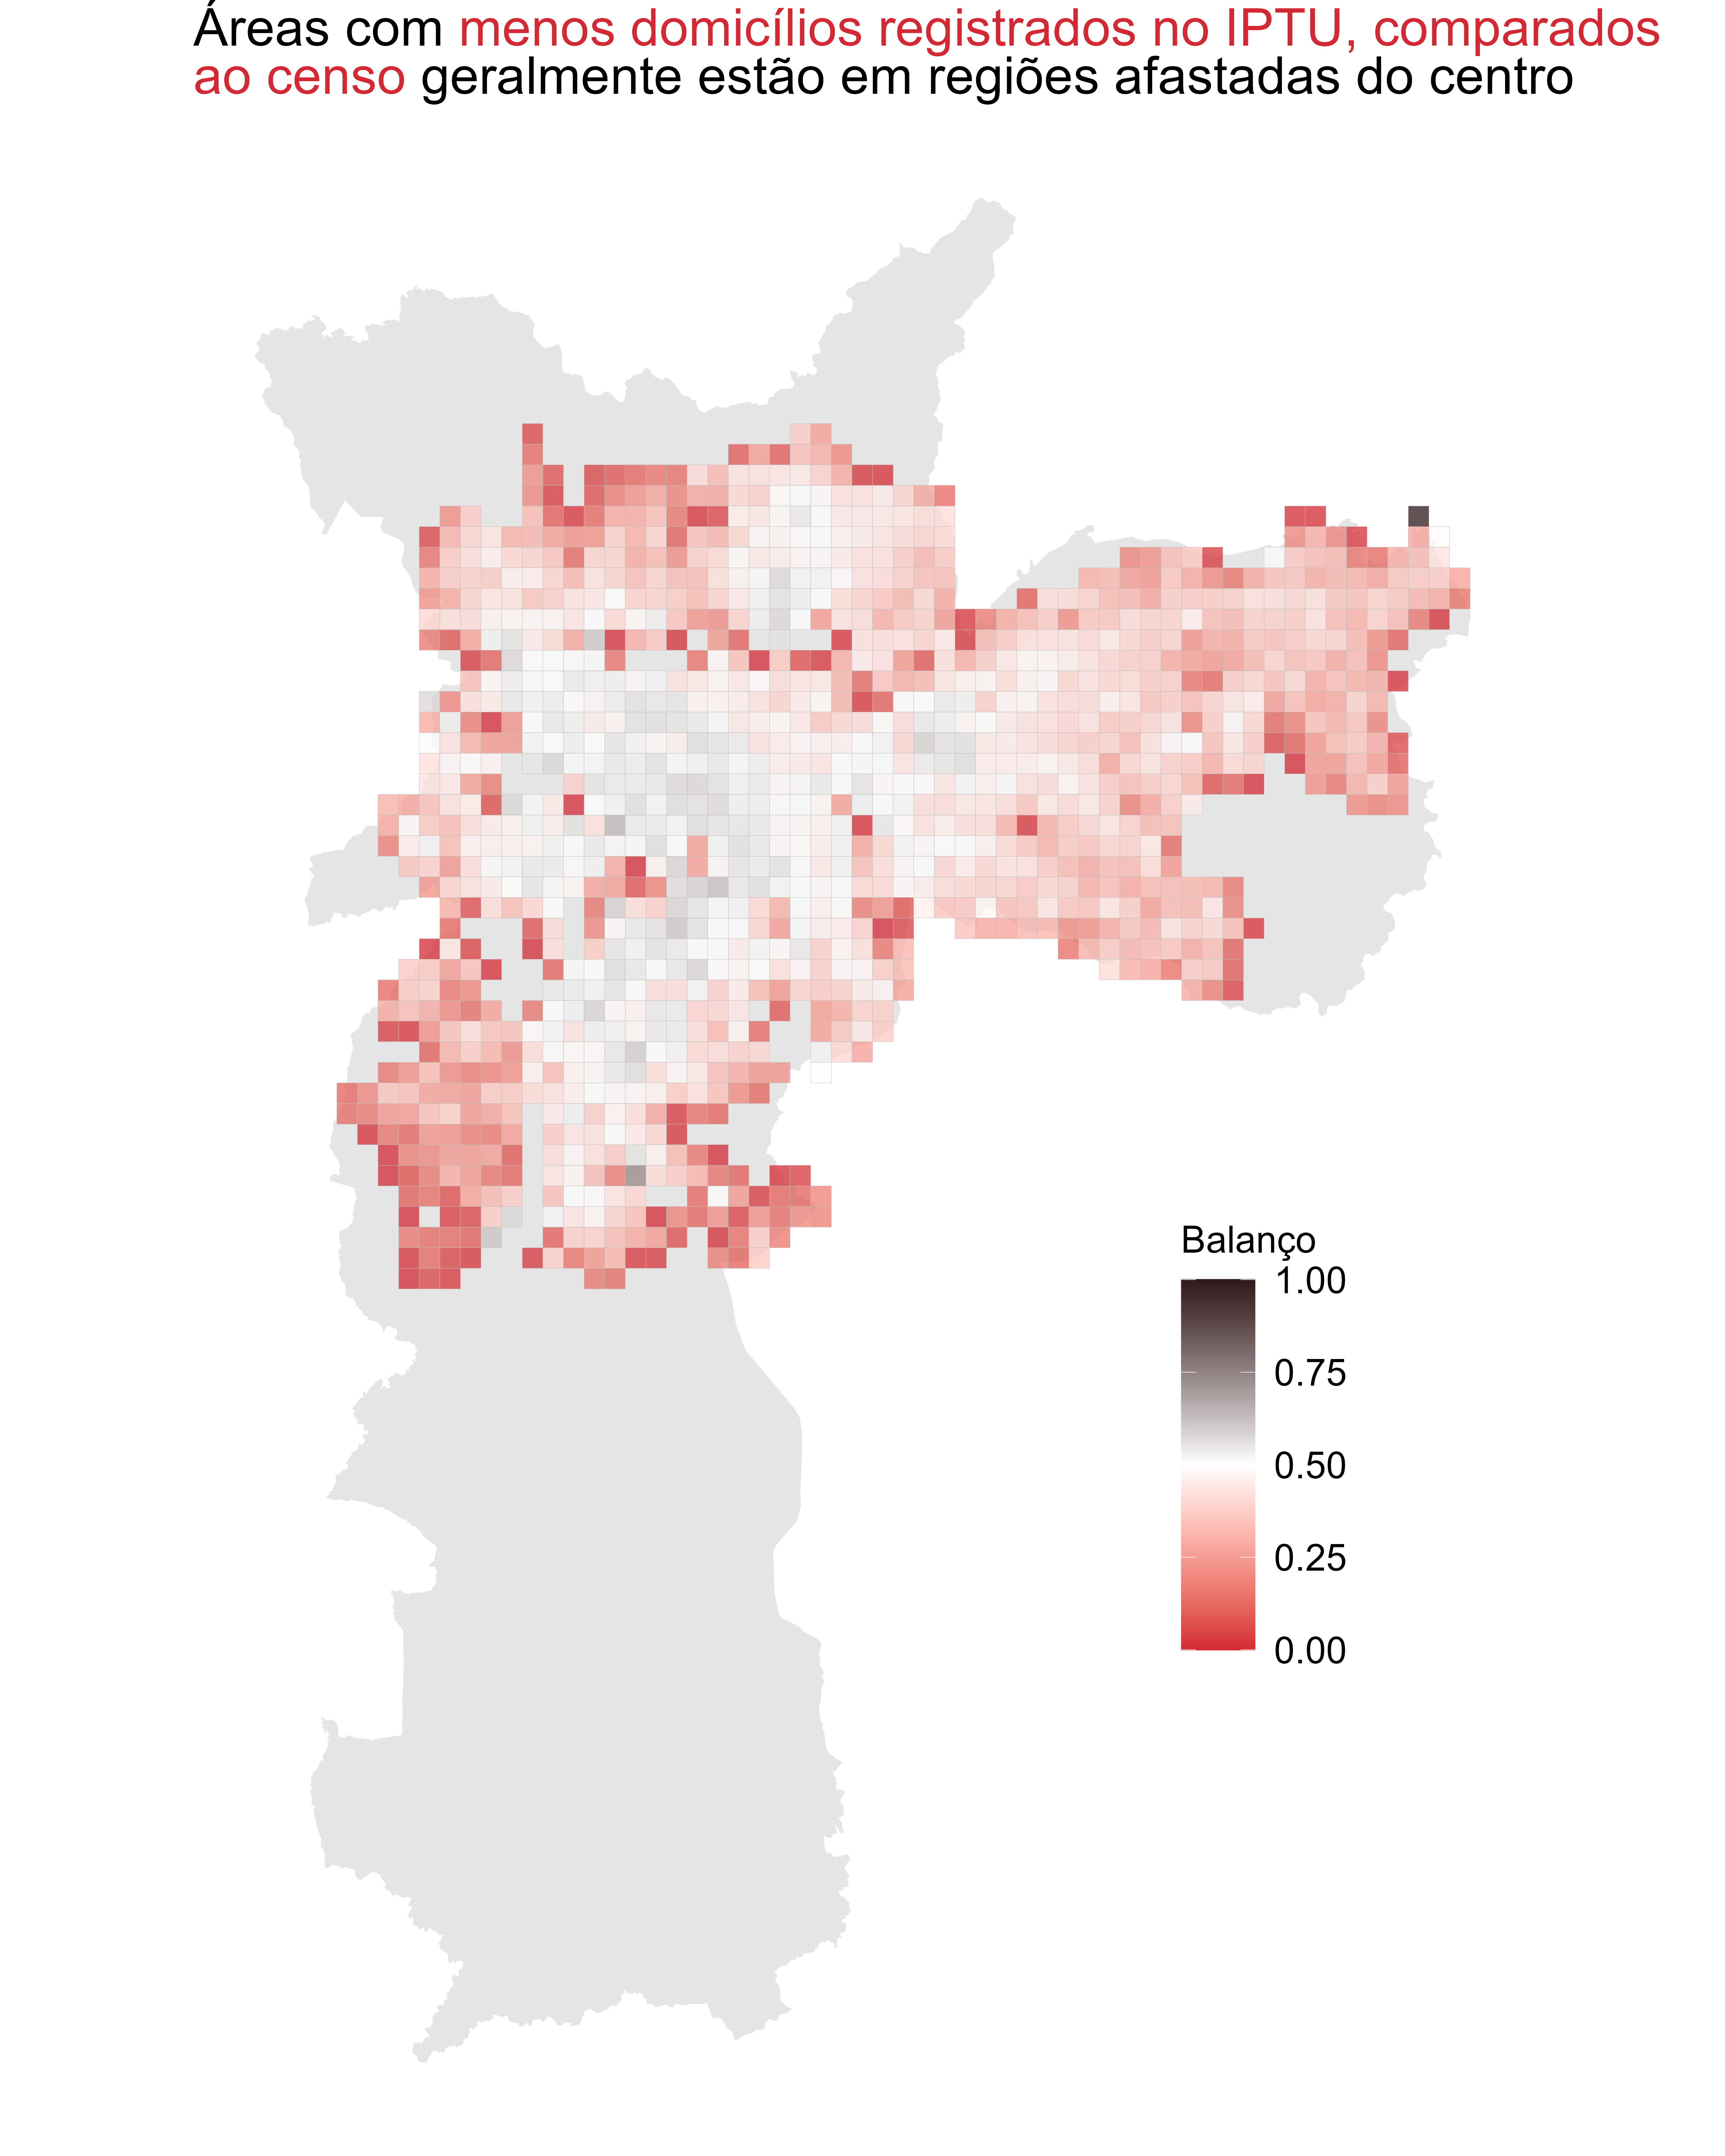
\includegraphics[width = \linewidth]{imagens/balanco_raster.png}
        \caption{Abordagem Raster}
        \label{fig:balanco-raster}
    \end{subfigure}
    \label{fig:erros-join}
\end{figure}

Com as bases relacionadas, é importante fazer um balanço para analisar se as informações batem. A única informação em comum entre as bases é o número de unidades habitacionais, que nos dados do IPTU são classificadas como unidades, e na do Censo como domicílios. A definição deles não é exatamente a mesma, porém é a única informação possível de ser validada. Caso o número de domicílios no Censo seja maior do que o de unidades no IPTU, é um forte indicativo de que há moradias irregulares. Para medir essa diferença, foi criado um indicador chamado balanço, que é construído a partir do número de unidades dividido pelo número de unidades mais domicílios. Caso o balanço seja próximo de 50\%, as informações são consistentes. Na medida em que o balanço se aproxima de 0\%, significa que há mais unidades no censo do que no IPTU, enquanto mais próximo de 100\% indica o contrário.

\begin{quote}
    ``Domicílio é o local estruturalmente separado e independente que se destina a servir de habitação a uma ou mais pessoas, ou que esteja sendo utilizado como tal. A separação fica caracterizada quando o local de habitação for limitado por paredes, muros ou cercas e coberto por um teto, permitindo a uma ou mais pessoas, que nele habitam, isolar-se das demais, com a finalidade de dormir, preparar e/ ou consumir seus alimentos e proteger-se do meio ambiente, arcando, total ou parcialmente, com suas despesas de alimentação ou moradia. A independência fica caracterizada quando o local de habitação tem acesso direto, permitindo a seus moradores entrar e sair sem necessidade de passar por locais de moradia de outras pessoas''\cite{IBGE2013}.
\end{quote}

No mapa da Figura \ref{fig:pontos_erro}, para cada setor censitário foram simulados pontos aleatórios dentro da geometria do setor para representar sua população. Nos setores censitários em que não há nenhum lote presente, ou seja, há uma subnotificação de imóveis na base do IPTU, os pontos foram pintados de vermelho. Em azul, estão as geometrias de lotes irregulares e favelas, disponibilizados no GeoSampa. É possível identificar que a maioria dos setores censitários que não possuem loteamento estão nessas áreas de lotes irregulares e favelas. Para analisar em termos numéricos, no histograma da Figura \ref{fig:balanco} é possível identificar que há diversos setores censitários com domicílios registrados, mas nenhuma unidade habitacional no IPTU. Ademais, são incomuns os casos em que são semelhantes os números de domicílios e unidades. Apesar de isso ser um problema do ponto de vista do planejamento da cidade, não é uma limitação para esta pesquisa, visto que os instrumentos de regulação não vão impactar estas áreas. Na Figura \ref{fig:balanco-raster}, um procedimento semelhante foi feito. Para cada célula do \textit{raster} foi calculado este indicador de balanço para analisar as inconsistências entre as bases. É notável que as células que se encontram em regiões centrais apresentam uma quantidade pequena de erros. Os casos mais críticos são células nas periferias.

\begin{figure}[h]
    \centering
    \caption{Diferença entre unidades e domicílios por setor censitário}
    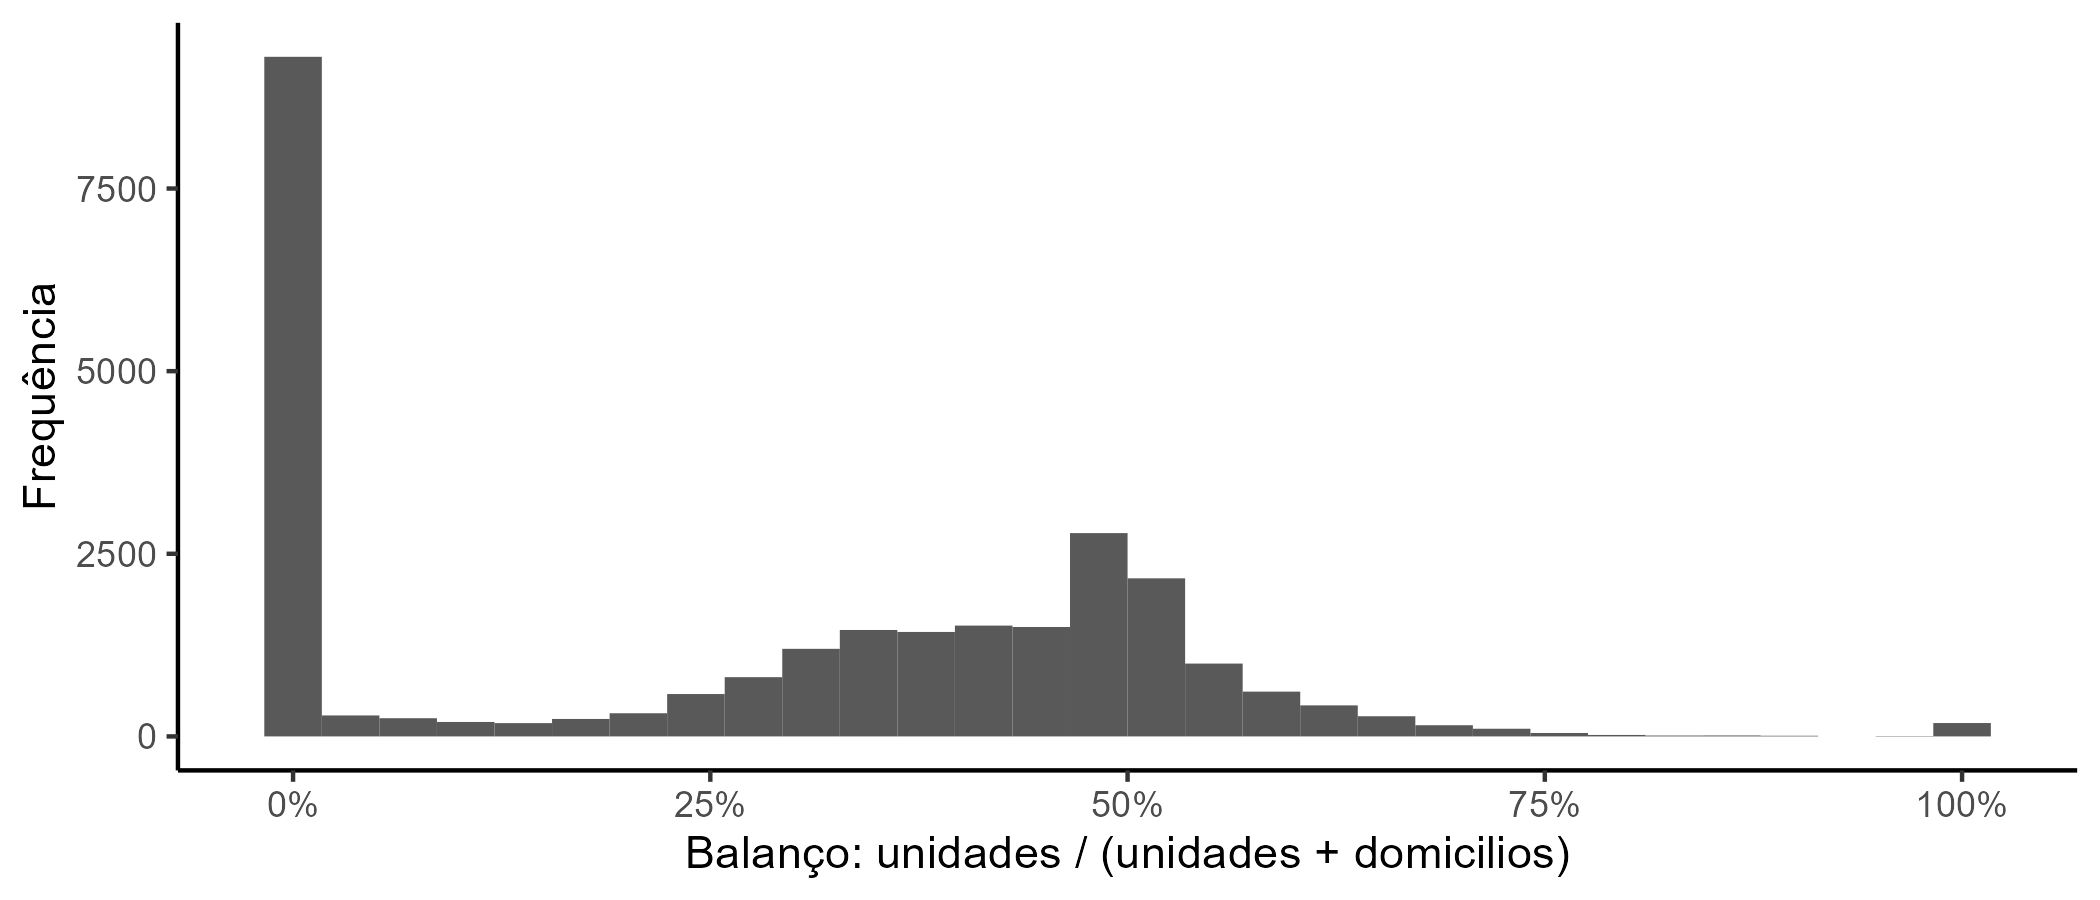
\includegraphics[width = \linewidth]{imagens/disparidade_censoIPTU.png}
    \label{fig:balanco}
\end{figure}

Na Figura \ref{fig:rasters} é possível analisar o perfil geográfico dos instrumentos regulatórios. Como é de se esperar, regiões com maior adensamento também apresentam maior CA, verticalização e menor cota parte. Dentre as 5 células com maior densidade, uma está no centro da cidade (Sé) e as outras quatro estão em favelas: duas em Paraisópolis, uma em Heliópolis e outra no distrito Pedreira da subprefeitura Cidade Ademar, onde há diversas pequenas favelas. 

\begin{figure}[h]
    \centering
    \caption{Rasters com os indicadores utilizados na regulação}
    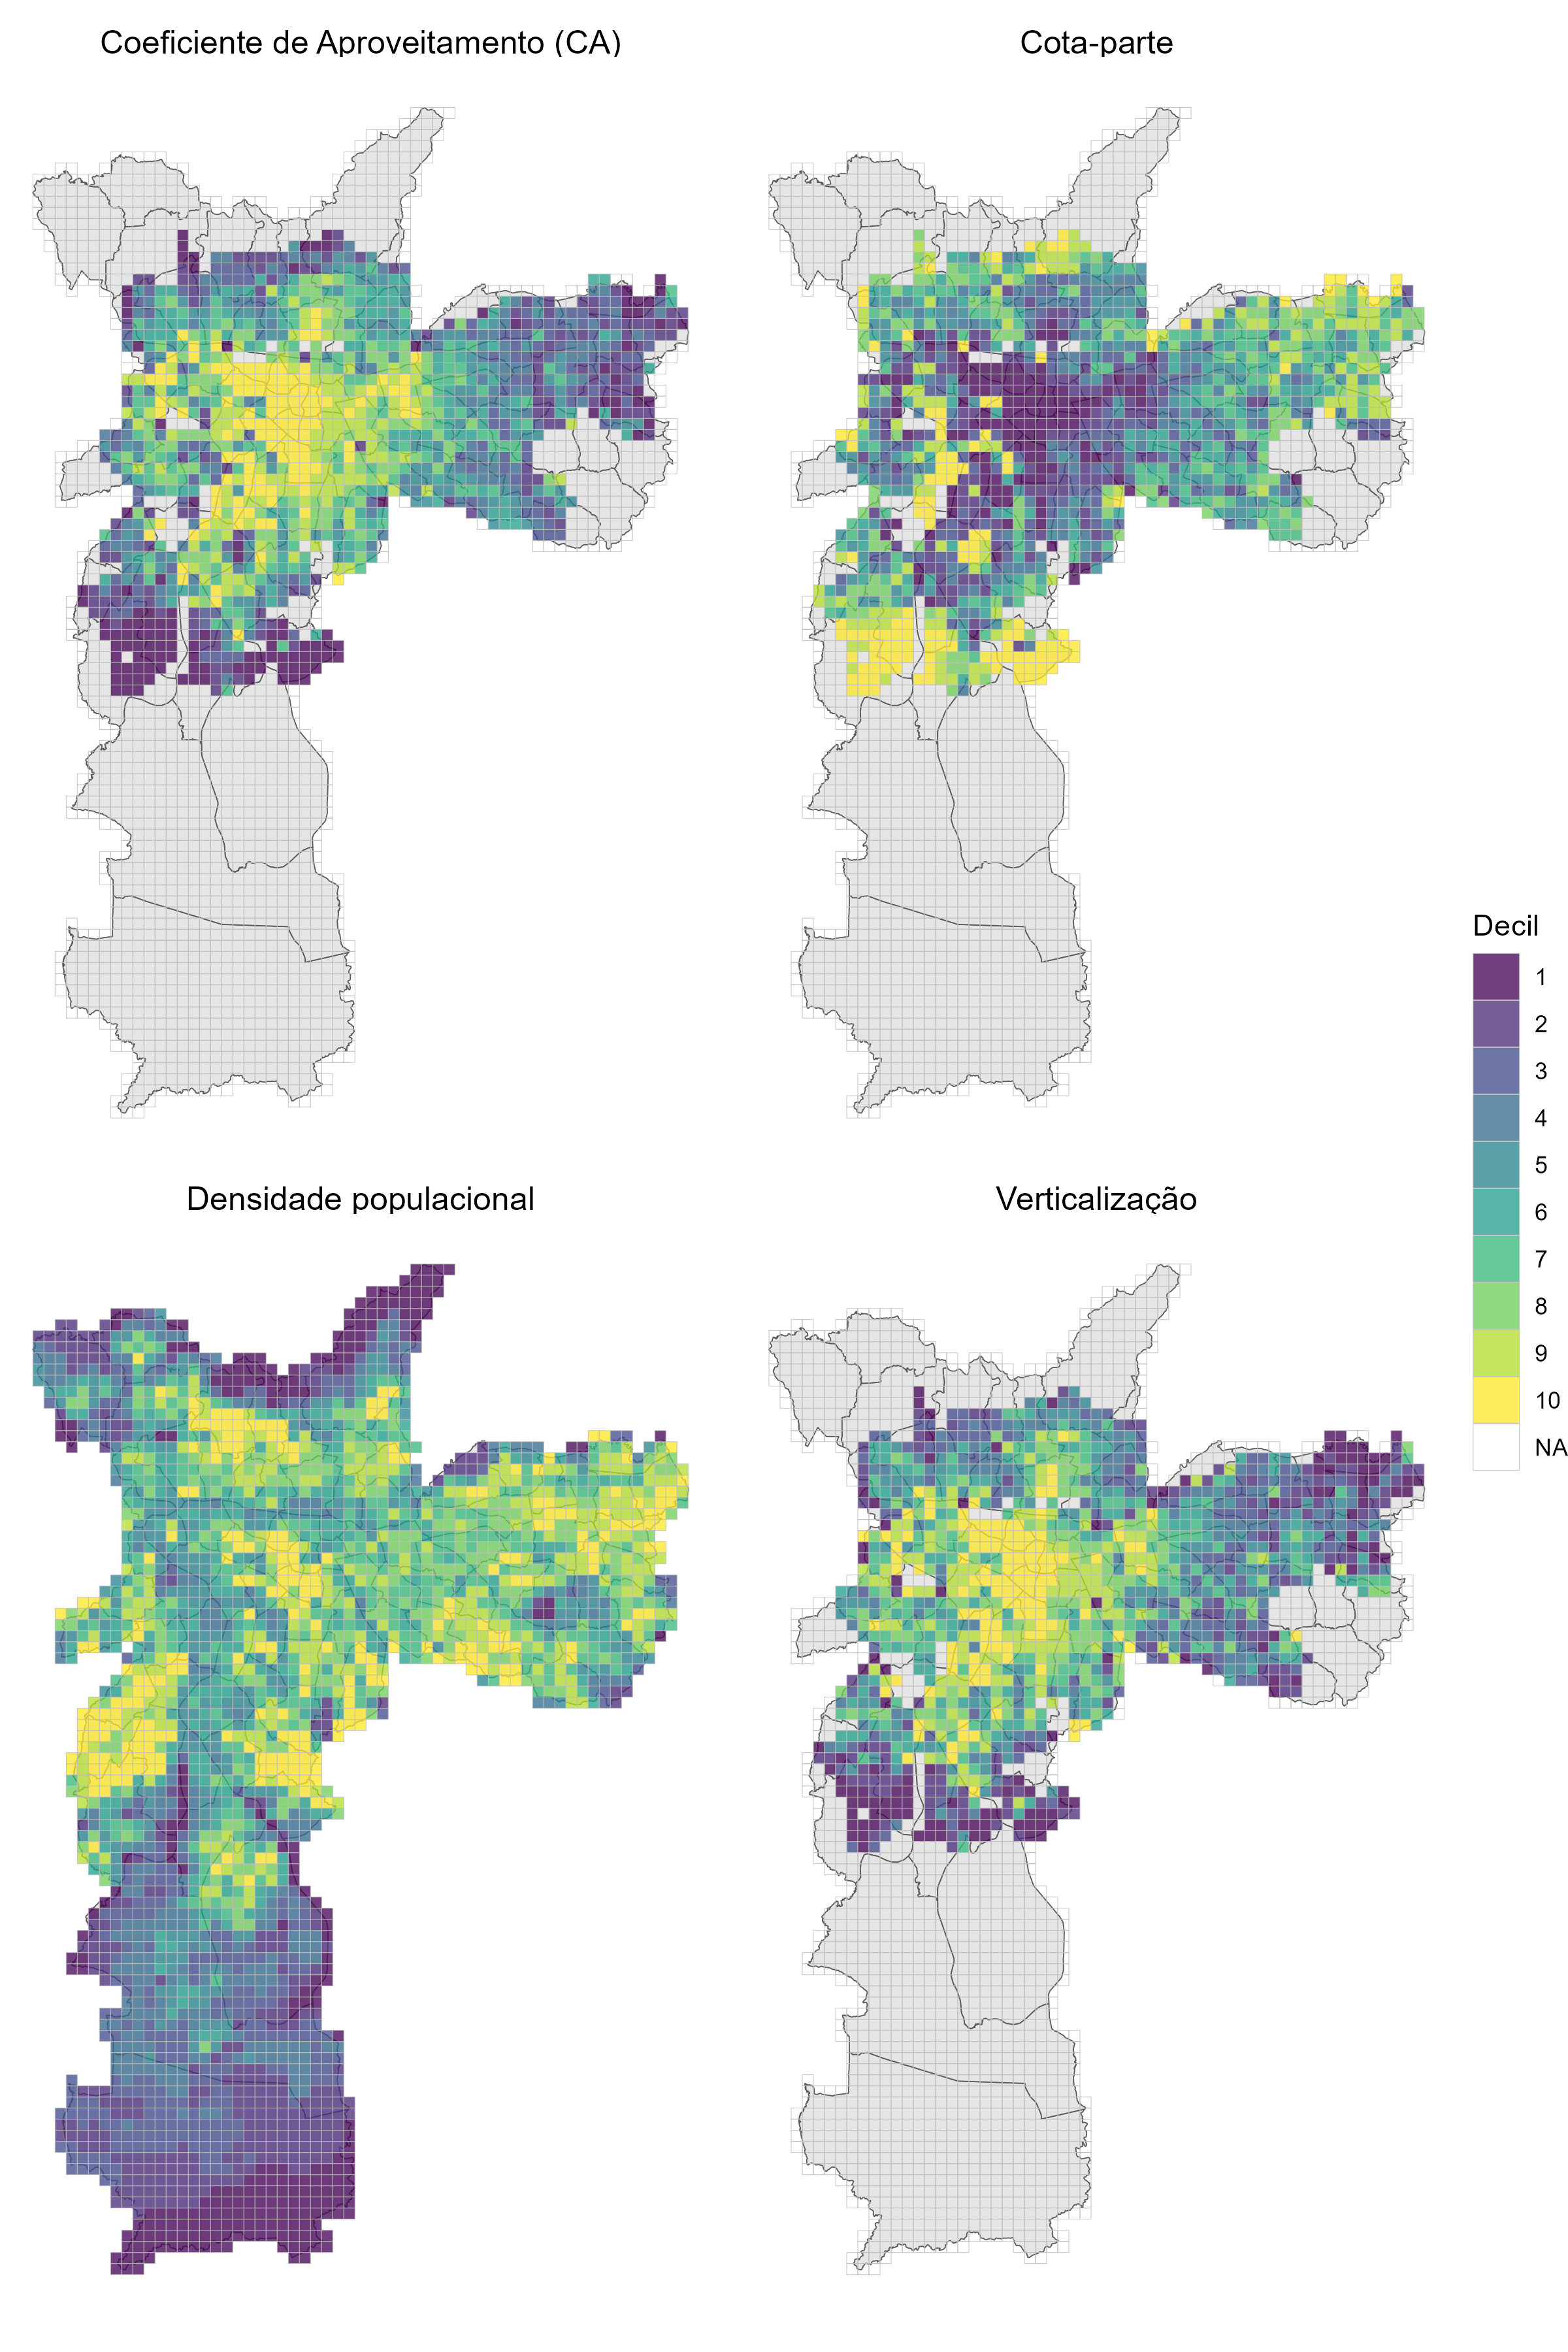
\includegraphics[width = \linewidth]{imagens/rasters.png}
    \label{fig:rasters}
\end{figure}

\section*{Alguns resultados preliminares}

Apenas através da análise descritiva já é possível concluir que em boa parte da cidade os instrumentos regulatórios não funcionam, visto que as moradias não estão nem registradas nos sistemas públicos. Dessa forma, não importa qual regra for adotada pelo governo, estas áreas não serão impactadas por isso. Em termos numéricos, dos 4.996.529 domicílios registrados pelo Censo, há apenas 3.096.719 unidades registradas no IPTU, o que representa um índice de moradia regular (em termos legais) de aproximadamente 61,98\%. Além disso, entre as regiões mais densas da cidade, muitas estão nestes 38\% que não estão registradas no IPTU, portanto há outras forças além da regulação que levam a esse adensamento.


\chapter{Análise}

Considerando o modelo microeconômico apresentado na Seção \ref{sec:micro}, a forma como a densidade é definida segue a Equação \ref{eq:emp-densidade}, na qual $D$ representa a densidade habitacional e $x$, a distância em relação ao centro. Os parâmetros $\alpha_0$ e $\alpha_1$ são importantes para capturar a magnitude do efeito da distância.

\begin{equation}
    D = \alpha_0\cdot e^{-\alpha_1\cdot x}
    \label{eq:emp-densidade}
\end{equation}

Para que o modelo seja estimável econometricamente, ele deve ser linear nos parâmetros, necessitando uma transformação logarítimica

\begin{equation}
    \ln{D} = \ln{(\alpha_0)} - \alpha_1\cdot x
\end{equation}